%; whizzy paragraph
%; whizzy-paragraph "^\\\\dancersection"
% -initex iniptex -latex platex -format platex -bibtex jbibtex -fmt fmt
% 以上 whizzytex を使用する場合の設定。

%     Tokyo Debian Meeting resources
%     Kansai Debian Meeting resources
%     Copyright (C) 2008 Junichi Uekawa
%     Copyright (C) 2008 Nobuhiro Iwamatsu

%     This program is free software; you can redistribute it and/or modify
%     it under the terms of the GNU General Public License as published by
%     the Free Software Foundation; either version 2 of the License, or
%     (at your option) any later version.

%     This program is distributed in the hope that it will be useful,
%     but WITHOUT ANY WARRANTY; without even the implied warranty of
%     MERCHANTABILITY or FITNESS FOR A PARTICULAR PURPOSE.  See the
%     GNU General Public License for more details.

%     You should have received a copy of the GNU General Public License
%     along with this program; if not, write to the Free Software
%     Foundation, Inc., 51 Franklin St, Fifth Floor, Boston, MA  02110-1301 USA

%   Pdf作成手順
% dvipdfmx debianmeetingresume2011-fuyu.dvi
%  preview (shell-command (concat "evince " (replace-regexp-in-string "tex$" "pdf"(buffer-file-name)) "&"))
% 画像ファイルを処理するためにはebbを利用してboundingboxを作成。
%(shell-command "cd image2012-fuyu; ebb *.png")


% progress memo:
% 2017/6-2017/11がマージ対象
% イベント等でない場合は理由を書くこと。
% 必要な変更点は FIXME で記録しています。

%%ここからヘッダ開始。

\documentclass[mingoth,a4paper]{jsarticle}
\usepackage{monthlyreport}
\usepackage[dvips]{xy} % for advi workaround. Bug #452044
\usepackage{ulem}
\usepackage{wrapfig}

% ページ調整のため部分的に2段組に
\usepackage{multicol}

\begin{document}

\begin{titlepage}
\thispagestyle{empty}

\hspace*{-2.5cm}

\includegraphics{image2012-natsu/gudeb.eps}\\
\\
\\
\rotatebox{10}{\fontsize{32}{32} {\gt 東京エリア/関西Debian勉強会}}

%\vspace*{-1.5cm}
\hspace*{11cm}
\includegraphics[height=6cm]{image200502/openlogo-nd.eps}\\
\vspace*{0.1cm}
\hfill あんどきゅめんてっど でびあん 2017年冬号 2017年12月29日 初版発行
\end{titlepage}

\newpage
\thispagestyle{empty}\mbox{}
\newpage

% section の代わりの環境 -- 改訂する。
\renewcommand{\dancersection}[2]{%
\newpage
あんどきゅめんてっど でびあん 2017年冬号
%
% top line
\vspace{0.1mm}\\
{\color{dancerlightblue}\rule{\hsize}{2mm}}

%
% middle text
%
\begin{minipage}[t]{0.6\hsize}
\color{dancerdarkblue}
\vspace{1cm}
\section{#1}
\hfill{}#2\\
\end{minipage}
\begin{minipage}[t]{0.4\hsize}
\vspace{-2cm}
\hfill{}
\includegraphics[height=8cm]{image200502/openlogo-nd.eps}\\
\vspace{-5cm}
\end{minipage}
%
%
{\color{dancerdarkblue}\rule{0.74\hsize}{2mm}}
%
\vspace{2cm}
}

\setcounter{page}{1}
\begin{minipage}[]{0.2\hsize}
 \definecolor{titleback}{gray}{0.9}
 \colorbox{dancerlightblue}{\rotatebox{90}{\fontsize{80}{80}
{\gt \color{dancerdarkblue}デビアン勉強会} }}
\end{minipage}
\begin{minipage}[]{0.8\hsize}
\hrule
\vspace{1mm}
\hrule
\setcounter{tocdepth}{1}
{\small
 \tableofcontents}
\vspace{1mm}
\hrule
\vspace{3cm}

\end{minipage}

% FIXME: 本文を追加すること。
%-------------------------------------------------------------------------------
\dancersection{Introduction}{DebianJP}
%-------------------------------------------------------------------------------

\subsection{東京エリアDebian勉強会}

 Debian勉強会へようこそ。これからDebianの世界にあしを踏み入れると
 いう方も、すでにどっぷりとつかっているという方も、月に一回Debianについ
 て語りませんか?

 Debian勉強会の目的は下記です。

\begin{itemize}
 \item \underline{Debian Developer} (開発者)の育成。
 \item 日本語での ``\underline{開発に関する情報}'' を整理してまとめ、アップデートする。
 \item \underline{場}の提供。
 \begin{itemize}
  \item 普段ばらばらな場所にいる人々が face-to-face で出会える場を提供
    する。
  \item Debian のためになることを語る場を提供する。
  \item Debianについて語る場を提供する。
 \end{itemize}
\end{itemize}

 Debianの勉強会ということで究極的には参加者全員がDebian Packageをがりがり
 と作るスーパーハッカーになった姿を妄想しています。情報の共有・活用を通し
 て Debianの今後の能動的な展開への土台として、 ``場'' としての空間を提供す
 るのが目的です。

\subsection{関西 Debian 勉強会}

 関西 Debian 勉強会はDebian GNU/Linux のさまざ
 まなトピック(新しいパッケージ、Debian 特有の機能の仕組、Debian 界隈で起
 こった出来事、などなど)について話し合う会です。

 目的として次の三つを考えています。
 \begin{itemize}
  \item MLや掲示板ではなく、直接顔を合わせる事での情報交換の促進
  \item 定期的に集まれる場所
  \item 資料の作成
 \end{itemize}

 それでは、楽しい一時をお楽しみ下さい。

%201709 kansai
% ---------------------------------------------------
\dancersection{Debian で Lisp を動かす}{油谷知岐}

\subsection{はじめに}

Lispという由緒正しきプログラミング言語があります.
原初のそれは1958年に現れ, 2017年現在で実に60年の歴史の中で洗練されてきた言語であり, Debianと同様に非常に自由なプログラミングを旨とする思想を持っています.
また, Debianパッケージとして提供されているLisp処理系も数多くあり, その親和性は低くないと考えられます. ここでは, そんな素晴らしい言語”Lisp”とはどんな言語なのかを簡単に説明します.

\subsection{Lispとは}

Lispという言語は, 御存知の通り, \b{Lis}t \b{P}rocessorから命名されたものです. この言語は, プログラム自体のデータ構造がリストであるなど, データ構造として「リスト」がプログラム全体で非常に重要な役割を果たしています. プログラム自体が, 「プログラム(ソースコード)」でありながら, 「(リスト構造を持った)データ」でもあるため, 自分自身を操作しやすいという特徴を持ちます.また再帰・条件分岐・GC・動的型付けなど, 現在のPG言語の多くが備える仕組みの先駆けとなっているという歴史も持っています. \vspace{1em}\\
この言語はプログラム全体で「():括弧」が多用される, 他の言語とは異なる見た目をしているように見えるため敬遠されがちなようです. しかし, 慣れるとむしろ括弧が目印になり, ソースコードの塊がわかりやすいなどの利点もある上に, 非常に自由度の高いコーディングを可能にするという利点もあります. \vspace{1em}\\
また, Lispという言語を代表する強力な仕組みの一つとして, プログラムを生成するプログラムを記述するマクロシステムが良く話題にのぼる. このあまりにも強力な仕組みもまた, Lispという言語を難解であるかのように感じさせる原因の一つになっているようです. 

\subsection{Lispの歴史}

Lispという言語は長い歴史の中で様々な処理系/仕様が「方言」として採択されており, 少しずつ変化しながら発展している. 
大まかな変化の系列はWikipediaのLispのページに以下のように記載されています.
いつの時代もLispがなくなることはなく, 形を変えて生き続けていることがわかります.

\pagebreak

\begin{figure}[htbp!]
\centering
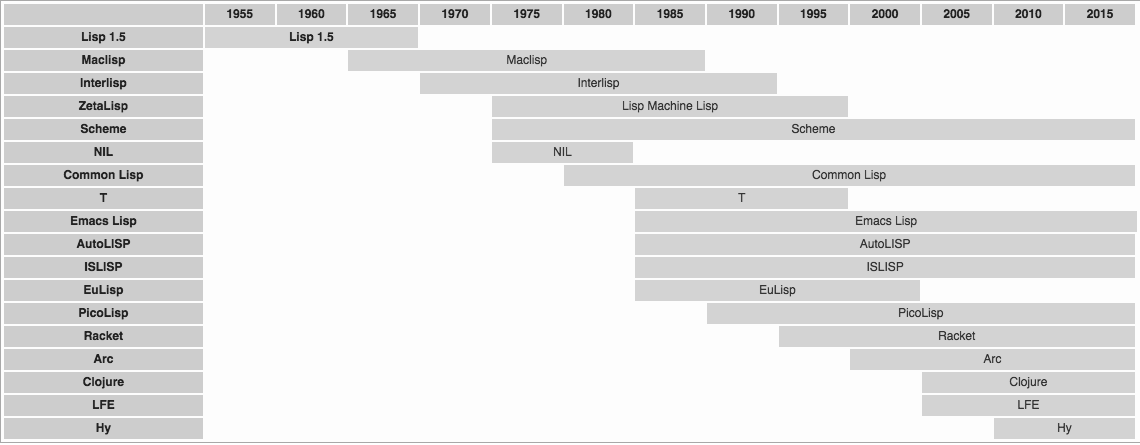
\includegraphics[width=\linewidth]{image201709-kansai/time-lines-lisp-dialect_gray.png}
\caption{Timelines of Lisp dialects (Wikipedia: Lisp(programming language)のページより}
\url{https://en.wikipedia.org/wiki/Lisp_(programming_language)}
\end{figure}

Lispは自己書き換えが容易であるという特徴のため, いわゆる人工知能の研究開発によく用いられていました.

\subsection{大まかなLisp方言の種類}

\subsubsection{代表的Lisp方言とその特徴}
表 \ref{table:lisp_dialect} に2017年現在で主流である6種類のLisp方言をまとめています. ただしこれらはあくまでもほんの一握りであり, 他にも現在動いているLisp方言は大量にあります. 

\begin{table}[htbp!]
\centering
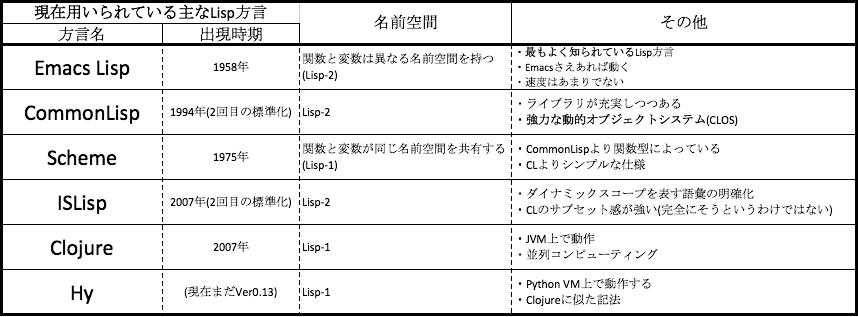
\includegraphics[width=\linewidth]{image201709-kansai/lisp-dial_gray.png}
\caption{現在主流なLisp方言}\label{table:lisp_dialect}
\end{table}

JVMやPythonVMで動くLisp, ErlangVMやその他様々な言語と連携するものや, 独自の機能を追加縮小したものなど, 現在でも新たな方言が活発に生まれています. 

表中の名前空間のカラムは, その方言がサポートする名前空間の扱いについて言及しています. Lispの方言には大きく2種類の名前空間の扱いがあります. 一つは, 関数名と変数名の名前空間を同一のものとして扱うLisp−1という枠組みです. こちらの名前空間では, 関数名と同じ名前の変数を宣言すると, 当然関数の定義が変数の定義に上書きされることになります. 具体的には以下のようになります. 

\begin{commandline}
;;; 関数定義
(define sample
	(lambda (x) (* x x)))

;;; 関数の評価
(sample 2)         ; 4

;;; 変数として?評価
sample             ; #<Closure>

;;; 変数の束縛
(define sample "It's a sample valiable")

;;; 変数の評価
sample             ; "It's a sample valiable"

;;; 関数として評価
(sample)           ; Error: "It's a sample valiable" is not a function [sample, *, sample]
\end{commandline}

一方, 関数名と変数名それぞれに異なる名前空間を用意するのがLisp-2と呼ばれる枠組みです. 実際には以下のように動作します. 

\begin{commandline}
;;; 関数定義 
(defun sample ()
	(format t "It's a sample function"))

;;; 関数の評価
(sample) ; It's a sample function
	     ; NIL

;;; 変数の評価
sample   ; Error

;;; 変数の束縛
(defparameter sample "sample parameter")

;;; 変数の評価
sample   ; "sample parameter"

;;; 関数の評価
(sample) ; It's a sample function
	     ; NIL
\end{commandline}

これらの違いからLisp-1/Lisp-2どちらが良いかといった考え方の違いが生まれたりします. 
私個人としてはLisp-2のほうが扱いやすいように感じています. 


\subsubsection{CommonLispとSchemeの代表的処理系}

表 \ref{table:cl_scm} には, Lisp方言の中でも現在最もよく使われている2大方言について, 幾つかの代表的な処理系を示します. Lispを学びはじめの時期は, 「処理系」と「方言」とを混同して考えがちな気がしますので, 簡単に説明しておきます. 
特にCommonLispとSchemeについては, 非常に多くの処理系が存在しますので, その中の一部を取り上げて説明します.\vspace{1em}\\ 
処理系それぞれに依存した機能が少なからず存在するため, プログラムの可搬性を考える場合は, 何がそれぞれに備わっていて, 何が無いのかを知っていることは望ましいです. とはいえ, 最近は処理系依存の部分をラップし, 違いを吸収してくれるライブラリが現れているので, それらを用いれば問題は軽減されるといえます. 

\begin{table}[htbp!]
\centering
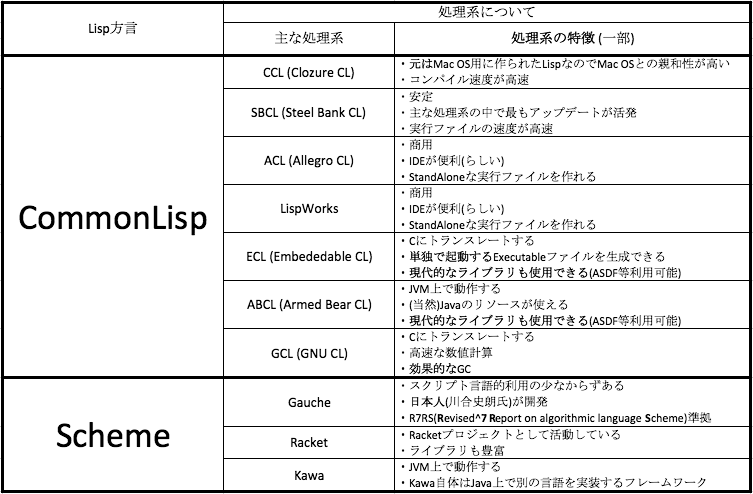
\includegraphics[scale=0.5]{image201709-kansai/cl-scm_gray.png}
\caption{現在主流なCommonLispとSchemeの処理系}\label{table:cl_scm}
\end{table}

\pagebreak

\subsubsection{Debianパッケージ内として提供されているLisp処理系}

CommonLisp
\begin{itemize}
\item SBCL
\item ECL
\item CMUCL
\item CLisp
\item GCL
\item CCL(バグあり)
\end{itemize}

Scheme
\begin{itemize}
\item mit-scheme
\end{itemize}


\subsection{Lisp界隈のライブラリ事情}
 Lisperは各自がオレオレライブラリを書くので, 使えるリソースが少ないのでは, というような声を耳にすることがあります. 実際, PythonやJavaに比べると, 相対的に少ないとは思いますが, 無いわけではありません. むしろ近年活発に開発が進んでいるようにも伺えます. 特にCommonLispは, 主にASDF(Another System Definition Facility)というライブラリ管理ライブラリを中心にしてできているQuickLispというパッケージマネージャの台頭によりライブラリの共有が進んでいます. Schemeの方は, CLに比べライブラリが少ないようです. 本稿ではCommonLispに焦点を絞って説明します. \vspace{1em}\\
CommonLispには, 正式な仕様として, ANSI Common Lispという仕様があります. この仕様の中で定義されているライブラリ管理システムは, 現在は非推奨であるはずの「Require/Provide」です. Emacs-Lispではよくお目にかかる方もいらっしゃるかと思います. 
しかし, 現在の主流としては, Require/Provideではなく, 上述のASDFというシステムがデファクトすアンダー度として使用されています. これをもとにしたパッケージマネージャがQuicklispです. \vspace{1em}\\
Quicklispに登録されているライブラリ数はQuickdocs \url{http://quickdocs.org} によると, 2017年9月現在で1557件あり, Web系(Webサーバー, パーサーやデータベースなど)や機械学習ライブラリ, GUIアプリケーション作成用ライブラリなどが多く見られます. 
まだ十分に整備されているとは言えませんが, これからのさらなる発展を考えれば, 実用に耐えるレベルである部分もあります. 

\subsection{Debian9でCommonLisp実行環境を構築する}

では, ここからは実際にLispをプログラムする環境をDebian9上に構築する手順を説明します. EmacsLispで良ければ当然, Emacsさえあれば完了なのですが, 今回はCommonLispの環境を整え, ライブラリを用いてプログラムが書けるようになるところまで進めます. ここではEmacsを使うことを前提として話を進めます. 

\subsubsection{処理系のインストール(今回はSBCL)}

まずは, CommonLispの処理系をインストールします. Debian Stretchからはパッケージマネージャとしてaptが推奨ですね. SBCLという処理系をaptからインストールします. 

\begin{commandline}
	~ $ sudo apt install sbcl slime cl-asdf
\end{commandline}
	
インストールが終われば既に, CommonLispを書き, 実行できる状況はできています. 実際に動くか試してみましょう. 

\begin{figure}[htbp!]
\centering
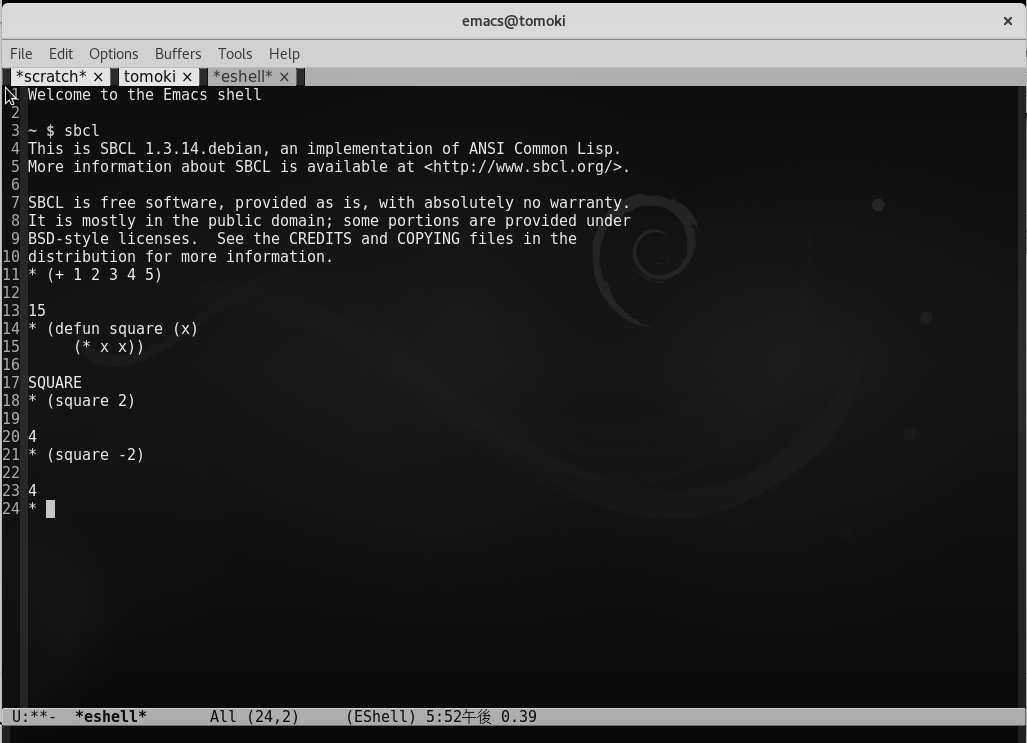
\includegraphics[width=\linewidth]{image201709-kansai/sbcl_gray.png}
\caption{SBCLの実行画面}
\end{figure}

正しく動作していれば次の作業に移ります. 

\subsubsection{統合開発環境のセットアップ}
この段階で, Lispプログラムを書き, 動かすことが可能になっていますが, 実際にコーディングするとなるとREPL上だけで作業するのは不便でしかありません. 
Emacsでは, SLIMEというCommonLispのための非常に便利な対話的開発ができるIDEを動かすことができます. 


\subsubsubsection{Emacsの設定ファイルの更新}
Emacsの設定ファイルである~/.emacsもしくは~/.emacs.d/init.elに以下の設定を追加し, SLIMEを使用可能にします. 


\begin{commandline}
(add-to-list 'load-path "/usr/share/common-lisp/source/slime/") ;; 自分の環境に合わせて変える
(setq inferior-lisp-program "/usr/bin/sbcl") ;; 自分の環境に合わせて変える
(require 'slime)
(slime-setup)
\end{commandline}


これらの設定を有効化して, "M-x slime"を実行しSlimeを起動します. 以下のような画面になれば成功です. 

\begin{figure}[htbp!]
\centering
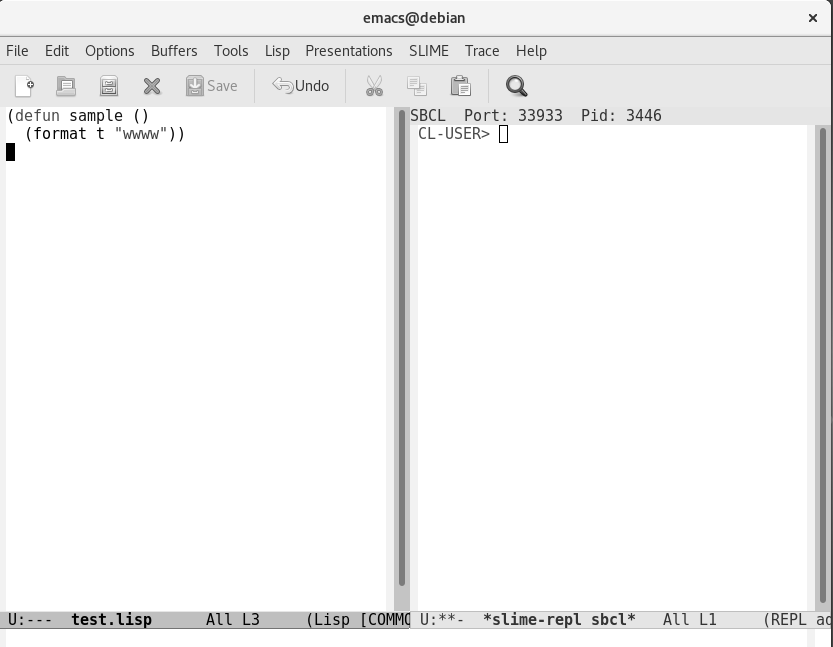
\includegraphics[width=\linewidth]{image201709-kansai/run-slime_gray.png}
\caption{SLIME起動画面}
\end{figure}

この画面では, 左側がLispソースファイル, 右側がREPLを示しています. 
SLIMEは, SwankサーバーというLispを処理するサーバにソケット通信で接続し, REPLを実現する仕組みになっている. なので, ターミナルなどで立ち上げたSwankサーバーがあれば, EmacsのSLIMEからそのサーバーにアクセスすることも可能です. 

\subsubsection{ライブラリ管理システムのインストール}

CommonLispにはQuicklispというライブラリ管理システムがあります. 以下のコマンドでインストールできます. 

\begin{commandline}
$ curl -O https://beta.quicklisp.org/quicklisp.lisp

$ curl -O https://beta.quicklisp.org/quicklisp.lisp.asc

$ gpg --verify quicklisp.lisp.asc quicklisp.lisp

$ sbcl --load quicklisp.lisp

* (quicklisp-quickstart:install)

* (ql:add-to-init-file)

* (quit)
\end{commandline}

QuicklispはLispで書かれており, インストールプログラムを処理系にロードして使用します. 上記のコマンドを実行すると, Homedir以下にquicklisp/.sbclrcというファイルができるはずです. これはSBCL用設定ファイルです. 上のコマンドではこの設定ファイルにQuicklispのロードを行うコードが追記されるため, 処理系起動時にはQuicklispが使用可能になっています. 

\subsubsection{プログラムの開発}
ここまでで十分に開発環境が整いました. これ以降の設定は各自の好みに合わせて変化させてください, それでは, 最後に, この環境でLispの環境を活かした高速な開発の手順を簡単に説明します. 
次のような簡単な関数をソースファイル側で定義します. 

\begin{commandline}
(defun sample ()
	(format t "It's a sample function"))
\end{commandline}

これを入力した後, この関数の中の何処かにマークをおいて, "C-c C-c"コマンドを打つことでREPLに送信し, コンパイルすることになります. 

\begin{figure}[htbp!]
\centering
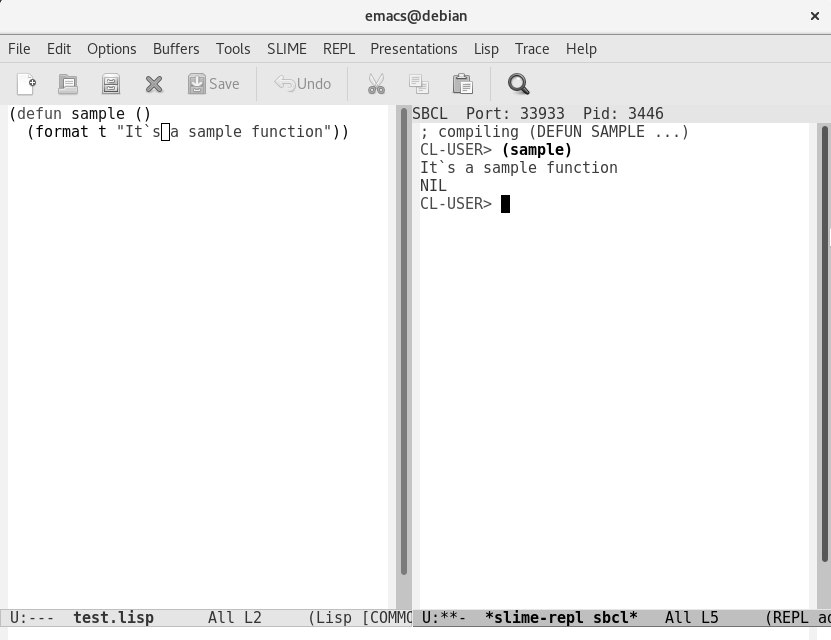
\includegraphics[scale=0.5]{image201709-kansai/do_gray.png}
\caption{関数の実行}
\end{figure}

この状態ですでにREPLの方でも関数が定義された状態になります. 
最後に定義した関数を実行してみます. 
正しく動いていることがわかります. 

\subsubsubsection{プログラムの開発2}
以降はファイルにLispプログラムをまとめて記述し, ファイル名を例えば「sample.lisp」といった名前にし, そのファイルを読み込みます. ファイル読み込みは以下に示すloadコマンドです. 

\begin{commandline}
(load "~/Desktop/sample.lisp")
; t
(sample)
; It's a sample function
\end{commandline}

ここまででLispでプログラムを書くための基本的な環境設定は整いました. 


\subsection{まとめ}
本稿では十分に記lesすことは叶いませんでしたが、Lispは上述のREPLをはじめとした、非常に効率のいい高速開発が可能な強力な言語です。
Common Lispなどは使用の中にリバースエンジニアリングのためのディスアセンブルの昨日や、最適化オプションをを持っており、C言語と比べても遜色のない実行速度のプログラムを書くこともできるよう設計されています。

マクロを用いた自己書き換えの能力なども相まって、人工知能的なプログラムを構築するのに有用であると考えられます。
そのシンプルで思考をそのまま起こした者に近くなる言語設計は、プログラムの基礎を知るためにも有用であると言え、現在はあまり大きな注目を集めいているとは言えませんが、今後もう一度日の目を見るときが来るかもしれません。

また、近年では、日本人デベロッパーが開発・保守しているRoswell\footnote{ロズウェル:https://github.com/roswell/roswell}というCommon Lispパッケージマネージャーが台頭し始めており、今回解説した公式の環境構築よりも非常にシンプルな環境構築や、実用的なシステム構築を可能にする仕組みが開発され続けています。

とはいえ、モダンなLisp開発のためのドキュメントを集めることは容易ではありません。情報を得るためには、Lisperたちが集まるコミュニティに参加し、交流することを強くおすすめします。

2017年現在では、関西では我々が運営している「関西Lispユーザ会\footnote{https://kansai-lisp-users.github.io/}」が3ヶ月に1度程度、関東では「Shibuya.lisp\footnote{https://lisp.connpass.com/}」というグループが毎月、Lispに関する勉強会を行っています。

Lispの知識や経験は問われず、LTを聞きに行くだけでもLispユーザが今、どのようなことに興味を持っているのかを知る良い機会になると思われます。


\pagebreak
% ---------------------------------------------------

%201709
%-------------------------------------------------------------------------------
\dancersection{初めてのキーサインパーティ}{ysaito}
%-------------------------------------------------------------------------------
%debianmeetingresume201709-presentation-ysaito.tex

初めてキーサインパーティに参加して、どこでつまづいたかお伝えします。

\subsection[containsverbatim]{Macからcaffを使おうとして}
Homebrew から消えてた
\begin{commandline}
$ brew search signing-party
 ==> Searching local taps...
 ==> Searching taps on GitHub...
 ==> Searching blacklisted, migrated and deleted formulae...
 signing-party was deleted from homebrew/core in commit e05298ad8a:
\end{commandline}


%\subsection{gpgのみでやってみよう}
%  %%BoundingBox: 0.00 0.00 362.83 272.13
%  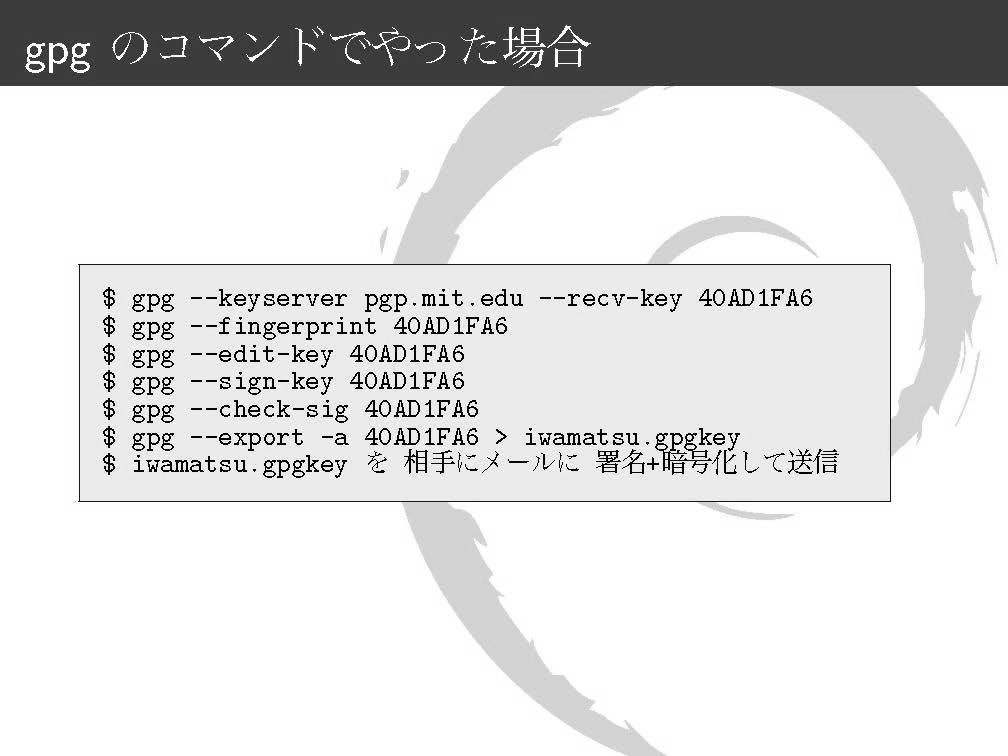
\includegraphics[width=0.8\hsize]{image201709/shiryo002_gray.jpg}
%
%

\subsection[fragile]{ではgpgのみでやってみようとして}
資料\footnote{http://tokyodebian.alioth.debian.org/pdf/debianmeetingresume201009-presentation.pdf}を参考に
gpgのみでやってみようとしてみたが、つまづいた
\\
相手の公開鍵で暗号化するところを自分の公開鍵で暗号化してしまった
\begin{commandline}
$ gpg --encrypt --recipient 相手の公開鍵ID 相手の公開鍵
\end{commandline}
  %%BoundingBox: 0.00 0.00 362.83 272.13
  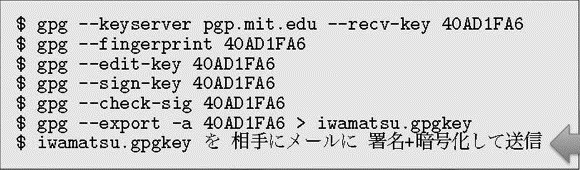
\includegraphics[width=0.8\hsize]{image201709/shiryo003_gray.jpg}

\clearpage
\subsection[containsverbatim]{caffをつかわないなら}
参考: https://github.com/thinkAmi/caffish-ps
\begin{commandline}
# キーサーバより相手の公開鍵を取得し、
# 自分の公開鍵の鍵束に入れる
$ gpg --keyserver pgp.mit.edu --recv-key 相手の公開鍵ID

# 表示されるフィンガープリントと、
# 手元の書類のフィンガープリントが一致していることを確認
$ gpg --fingerprint 相手の公開鍵ID

# 相手の公開鍵に署名
$ gpg --sign-key 相手の公開鍵ID

# 署名した公開鍵をエクスポート
$ gpg --export -a 相手の公開鍵ID > ./foo.gpgkey

# 自分の秘密鍵で署名した相手の公開鍵を、相手の公開鍵を使って暗号化
$ gpg --no-auto-check-trustdb  --trust-model=always \
  --armor --recipient 相手の公開鍵ID --encrypt ./foo.gpgkey
# foo.gpgkey.asc が生成される
# 暗号化した公開鍵をメールに添付し、
# メール本文を暗号化して相手へ送信
\end{commandline}
\noindent
これは面倒です。そうだ caff 使おう。
\\
Debian strech に caff をいれて
\\
メールサーバを立てて...
  
\subsection[fragile]{もう一つ詰まったところ}
  \begin{commandline}
$ caff -u 自分の公開鍵ID 一人目の公開鍵ID 二人目の公開鍵ID...
[NOTICE] Fetching keys from pool.sks-keyservers.net, this may take a while...
[WARN] Local-user 自分の公開鍵ID is not defined as one of your keyid in ~/.caffrc (it will not be used)
[ERROR] None of the local-user keys seem to be known as a keyid listed in ~/.caffrc
  \end{commandline}
~/.caffrc はちゃんと設定しているはずだけど...
\\
自分の公開鍵のフィンガープリントの後半16桁
  \begin{commandline}
$ caff 一人目の公開鍵ID 二人目の公開鍵ID...
  \end{commandline}
通った
  
%\subsection{参考にした資料}
%  キーサインパーティで参考にさせていただいた資料\footnote{http://tokyodebian.alioth.debian.org/pdf/debianmeetingresume201009-presentation.pdf}

  %%BoundingBox: 0.00 0.00 362.83 272.13
%  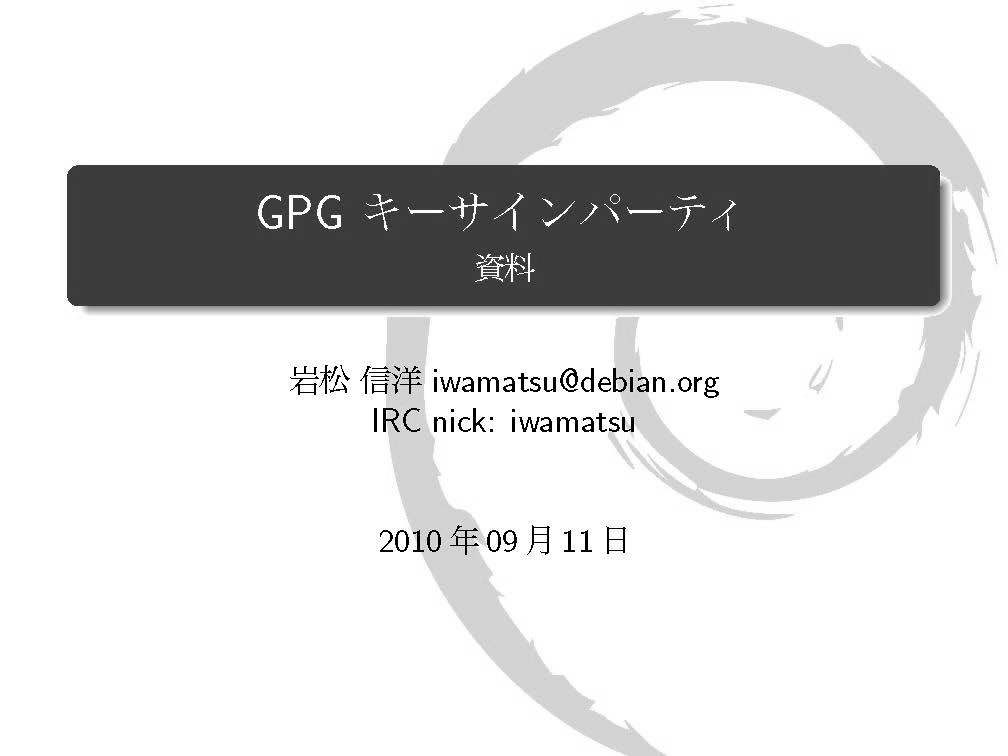
\includegraphics[width=0.8\hsize]{image201709/shiryo001_gray.jpg}

%201710
%-------------------------------------------------------------------------------
\dancersection{caffとmail-transport-agent}{yy\_y\_ja\_jp}
%-------------------------------------------------------------------------------
%debianmeetingresume201710-presentation-yyoshino.tex

キーサインに便利なcaffとそれに使うmail-transport-agentについて解説します。

\subsection{caff}
\begin{itemize}
 \item caff(1) -- CA - Fire \& Forget

 キーサインパーティなどで便利なツール

 \item 
 signing-party パッケージでインストールできる

 \item 
 キーサインパーティに参加した後で、このコマンドを実行すれば必要な作業をやってくれる

 

 \begin{enumerate}
  \item 参加した人の公開鍵を取得
  \item その公開鍵に自分の秘密鍵で署名
  \item 署名済みの公開鍵をその人にメールで送信
 \end{enumerate}

\end{itemize}
  


\subsection{Mail Transport Agent}
 メール転送エージェント (MTA)
は、
 受け付けたメッセージを他のサーバなどに転送するプログラムです。ここで
 
 \begin{itemize}
  \item 受け付けかた(インターフェース)には
	\begin{itemize}
	 \item SMTP(TCP 25番ポートなど)
	 \item sendmail互換(/usr/sbin/sendmailコマンドを実行して標準入力に
	       渡すなど)
	 \item など
	\end{itemize}
 があり、
  \item 転送のしかたには
	\begin{itemize}
	 \item 自力でDNSを引いて送付先サーバに転送
	 \item 他のサーバに渡して転送してもらう(リレー)
	\end{itemize}
	があります。
 \end{itemize}
 


 受け付けかた(インターフェース)については、
 メッセージをマシン上にある(ローカル)MTAに
	       渡すだけなら、わざわざメールサーバ(SMTPサーバ)を立ち上
 げてそれ経由で渡す必要はありません。
 /usr/sbin/sendmailコマンドを起動して、
 そのコマンド自体が転送してくれれば充分です。


次に転送のしかたですが、
 自力で転送してしまうと次のような様々な問題が起こります。
 
 \begin{itemize}
  \item そのメールサーバをインターネット公開にしていない場合は自分宛てのメー
	ルが受信できない -- エラーメールも受け取れない
  
  \item 自分のメールアドレスのドメインがそのサーバ管理でない場合はなりす
	まし(フィッシング)になってしまう

参考: このようなメールが届いたときにGoogleメールが表示することがある警告メッセージ
	\begin{quote}
This message may not have been sent by: xxx@example.com
	\end{quote}
\begin{quote}
Why is this message in Spam? It's similar to messages that were detected by our spam filters.
\end{quote}
  
  \item OP25B の影響で送信できないこともある
 \end{itemize}



\subsection{mail-transport-agent}


\begin{itemize}
 \item Debianポリシーで定められた仮想パッケージのうちの1つ

% \scriptsize
 \verb|/usr/share/doc/debian-policy/virtual-package-names-list.txt.gz|
% \footnotesize
 \url{https://www.debian.org/doc/packaging-manuals/virtual-package-names-list.txt}
% \normalsize
 で見られる

\begin{verbatim}
 mail-transport-agent    a mail transport agent (e.g. Smail, Sendmail, &c)
\end{verbatim}

 \item 
 mail-transport-agent を提供しているパッケージは
 \verb|apt-cache showpkg mail-transport-agent|
 や
% \footnotesize
 \url{https://packages.debian.org/stable/mail-transport-agent}
% \normalsize
 で見られる
\end{itemize}



 \begin{itemize}
  \item Debianのデフォルトは exim4-daemon-light\\
	-- 仮想パッケージ default-mta も提供(Provides)
 \item どのパッケージも Conflicts: mail-transport-agent, Replaces:
       mail-transport-agent, Provides: mail-transport-agent と書いてある\\
       ⇒ 2つ以上インストールできないようになっている
 \end{itemize}

\begin{commandline}
$ apt-cache show exim4-daemon-light
Package: exim4-daemon-light
Source: exim4
Version: 4.89-2+deb9u1
Installed-Size: 1167
Maintainer: Exim4 Maintainers <pkg-exim4-maintainers@lists.alioth.debian.org>
Architecture: amd64
Replaces: exim4-base (<= 4.61-1), mail-transport-agent
Provides: default-mta, exim4-localscanapi-2.0, mail-transport-agent
Depends: exim4-base (>= 4.89), libc6 (>= 2.16), libdb5.3, libgnutls30 (>= 3.5.6), libpcre3, debconf (>= 0.5) | debconf-2.0
Conflicts: mail-transport-agent
\end{commandline}

 \begin{itemize}
 \item MTAのパッケージが2つに分かれていることもある --
       mail-transport-agentを提供するパッケージがsendmail互換インターフェー
       ス(/usr/sbin/sendmail)などを提供
 \end{itemize}

\begin{commandline}
$ apt-cache show msmtp-mta
Package: msmtp-mta
Source: msmtp
Version: 1.6.6-1
(略)
Replaces: mail-transport-agent
Provides: mail-transport-agent
Depends: msmtp
Conflicts: mail-transport-agent
Description-en: light SMTP client with support for server profiles - the regular MTA
(以下略)

\end{commandline}
\begin{commandline}

$ apt-cache show msmtp
Package: msmtp
Version: 1.6.6-1
(略)
Depends: libc6 (>= 2.22), libgnutls30 (>= 3.5.6), libgsasl7 (>= 1.1), debconf (>= 0.5) | debconf-2.0, ucf
Recommends: ca-certificates
Suggests: msmtp-mta
Description-en: light SMTP client with support for server profiles
(以下略)

\end{commandline}

MTAがSMTPサーバも提供するかどうかはそのパッケージのプログラム次第です。

 \begin{itemize}
  \item SMTPサーバも提供する -- exim4-daemon-light, postfix, nullmailer
	など
  \item SMTPサーバを提供しない(リレー専用) -- msmtp など
 \end{itemize}


\subsection{caff と mail-transport-agent}
caff は署名済みの公開鍵をその人にメールで送信します。しかし 

 \begin{itemize}
  \item 実行されたマシン上にある(ローカル)MTA を使ってメール送信している
  \item デフォルトの MTA だとローカル配送のみ
 \end{itemize}
なのでそのままだと次のようなエラーメールになってしまいます。
\begin{verbatim}
Subject: Mail delivery failed: returning message to sender
(略)
	 Mailing to remote domains not supported
\end{verbatim}

	これは、メールがインターネットに出ていかない状態になっているためで、MTA
	の設定が必要です。

        もし自分の(uidに使っている)メールアドレスが自分の管理するメー
       ルサーバのドメインでないのなら(例えば \verb|@gmail.com| などの場合)、

 \begin{itemize}
  \item メールサーバ(SMTPサーバ)なし
  \item リレー専用
 \end{itemize}

       なMTAを選べば設定がかんたんです。
       例として msmtp-mta パッケージがあります。
設定については \url{https://wiki.debian.org/msmtp} をご覧ください。

 \begin{itemize}
  \item  個人の設定ファイル \textasciitilde/.msmtprc にGmailアカウントとSMTPサーバの情報を書いてリレー
 する方法が書かれている
  \item  パスワードをGPG鍵で暗号化して保存する方法も書かれている
 \end{itemize}



\subsection{まとめ}
\begin{itemize}
 \item caff はローカルのMTAを使ってメール送信する
 \item ローカルのMTAはmail-transport-agent仮想パッケージを提供するパッケー
       ジをインストールすればよい
 \item マシンにはmail-transport-agent仮想パッケージを提供するパッケージのうち
       1つだけをインストールできる(Conflicts/Replaces/Provides)
 \item MTAのパッケージが2つに分かれていることもある(msmtp/msmtp-mta,
       qmail/qmail-runなど)
 \item MTA にはSMTPだけでなくsendmail互換インターフェースもある -- caff作業マシンが
       インターネット公開のメールサーバでないならSMTPは不要
 \item 自分が管理していないドメインのメールアドレスなら、その外部SMTPサー
       バにリレーするようにローカルのMTAをインストール(msmtp-mta パッケー
       ジがおすすめ)し設定するとよい
\end{itemize}

%Debian / Ubuntu ユーザーミートアップ in 札幌 2017.07
\dancersection{lxcについて}{杉本 典充}
%debianmeetingresume201707-meetup-sapporo-presentation-sugimoto.tex

%\subsection{}

\subsection{アジェンダ}
  \begin{itemize}
  \item 自己紹介
  \item 仮想化技術について
  \item lxcとは
  \item lxcのインストール
  \item lxcのコマンド解説
  \item lxcを実用する
  \item おわりに
  \item 参考資料
  \end{itemize}



\subsection{自己紹介}
  \begin{itemize}
  \item Norimitsu Sugimoto (杉本 典充)
  \item dictoss@live.jp
  \item Twitter: @dictoss
  \item Debian-3.1、FreeBSD-6.2の頃から使っています
  \item Debian GNU/kFreeBSDが気になっておりウォッチ中
  \item 仕事はソフトウェア開発者をやってます
  \end{itemize}



\subsection{仮想化技術について}

\subsection[containsverbatim]{仮想化技術の分類}
  \begin{itemize}
  \item コンテナ型仮想化
  \item 準仮想化型
  \item 完全仮想化型 (エミュレーション型)
  \item 完全仮想化型 (ハイパーバイザ型)
  \end{itemize}


\subsection[containsverbatim]{仮想化技術のメリット・デメリット}
  \begin{itemize}
  \item 準仮想化型、完全仮想化型
    \begin{itemize}
    \item 物理マシンをエミュレートした仮想マシンとして動作する
    \item 仮想マシン上でもカーネルを動作させる
    \item 物理マシンで動かしていたプログラムはほぼそのまま動く
    \item CPU、メモリ、ディスクを多く消費する
    \end{itemize}
  \item コンテナ型仮想化
    \begin{itemize}
    \item ゲスト環境の動作にカーネルは不要(ホスト環境のカーネル上で動作)
    \item ゲスト環境は、ホスト環境から見るとプロセスとして扱われる
    \item ゲスト環境が利用できるリソースに制約がつく場合がある
    \end{itemize}
  \end{itemize}


\subsection[containsverbatim]{chroot}
  \begin{itemize}
  \item chrootシステムコールとchrootコマンド
  \item 1982年にビル・ジョイが開発したとされている
  \item \# chroot rootfsdir でコンテナ環境に入れることができる
  \end{itemize}





\subsection[containsverbatim]{lxcとは}
  \begin{itemize}
  \item LinuX Containersのことで、省略してlxcと読んでいる
  \item あるディレクトリ配下に実行ファイル、ライブラリ、設定ファイルを適切に配置したrootfsを準備する
  \item rootfsをchroot環境で起動し、仮想マシンのように動かすことができる
  \item Debian 9 Stretch では lxc-2.0.5 を採用
  \end{itemize}



\subsection{lxcのインストール}

% https://wiki.debian.org/LXC/LibVirtDefaultNetwork
\subsection[containsverbatim]{インストールの流れ}
  \begin{itemize}
  \item ブリッジネットワークとlibvirtdの準備
  \item lxcのインストール
  \end{itemize}



\subsection[containsverbatim]{ブリッジネットワークとlibvirtdの準備}

パッケージのインストール
\begin{commandline}
  # apt-get install libvirt-clients \
  libvirt-daemon-system ebtables dnsmasq
\end{commandline}

仮想ネットワークの設定
\begin{commandline}
  # virsh net-autostart default
  # virsh net-start default
\end{commandline}




\subsection[containsverbatim]{ブリッジネットワークとlibvirtdの準備}
確認
\begin{commandline}
  $ sudo virsh net-info default
  Name:           default
  UUID:           78564864-f237-4059-a12a-3ec04369a27b
  Active:         yes
  Persistent:     yes
  Autostart:      yes
  Bridge:         virbr0
  
  $ ip a show virbr0
  →192.168.122.1/24 が付与されている
\end{commandline}




\subsection[containsverbatim]{lxcのインストール}
  コンテナ内のリソース制約を処理するcgroupの確認
  \begin{commandline}
    # mount | grep cgroup
    →stretchは標準でmountされている
  \end{commandline}
  パッケージのインストール
  \begin{commandline}
    # apt-get install lxc libvirt0 libpam-cgroup \
    libpam-cgfs
  \end{commandline}
  環境を確認
  \begin{commandline}
  $ ls /usr/bin | grep lxc
  # lxc-checkconfig
  \end{commandline}


\subsection[containsverbatim]{lxcのインストール}
  \begin{itemize}
  \item lxc-create
  \item lxc-destroy
  \item lxc-start
  \item lxc-stop
  \item lxc-console
  \item lxc-attach
  \end{itemize}



\subsection{lxcのコマンド解説}

\subsection[containsverbatim]{lxc-create(1)}
  \begin{commandline}
    # lxc-create -n demo1 -t debian -- \
    --release=stretch --arch=amd64 \
    --mirror=http://ftp.jp.debian.org/debian
  \end{commandline}   
  \begin{itemize}
  \item 実行するとテンプレートがdebianの場合はdebootstrapを実行してrootfsをダウンロードする
  \item lxcのゲスト環境のディレクトリは、/var/lib/lxc/''コンテナ名'' 。中身は以下。
    \begin{itemize}
    \item config (設定ファイル)
    \item rootfs (コンテナの中身)
    \end{itemize}
  \end{itemize}


\subsection[containsverbatim]{lxc-create(2)}
  \begin{itemize}
  \item configを修正して、ネットワークの設定を行う
  \item lxc.network.type = veth
  \item lxc.network.flags = up
  \item lxc.network.link = virbr0
  \item lxc.network.name = eth0
  \item lxc.network.ipv4 = 192.168.122.60/24
  \item lxc.network.ipv4.gateway = 192.168.122.1
  \end{itemize}


\subsection[containsverbatim]{lxc-destroy}
  \begin{commandline}
  # lxc-destroy -n demo1
  \end{commandline}
  \begin{itemize}
  \item コンテナを削除します
  \end{itemize}


\subsection[containsverbatim]{lxc-start}
  \begin{commandline}
  # lxc-start -n demo1
  \end{commandline}
  \begin{itemize}
  \item 実行して何もエラーが表示されなければ、バックグラウンドでlxcコンテナが動き出します
  \item 起動したコンテナへの接続は、後述するlxc-consoleまたはlxc-attachで行います
  \item コンテナへのログインはsshでもログインできますが、ユーザを作成する必要があります
  \end{itemize}


\subsection[containsverbatim]{lxc-stop}
  \begin{commandline}
  # lxc-stop -n demo1
  \end{commandline}
  \begin{itemize}
  \item コンテナ環境を終了するよう指示を出します
  \item コンテナ環境の終了とは、コンテナ内のinitプログラムを終了することをいいます
  \item コンテナ環境でshutdown命令は実行できません
  \end{itemize}


\subsection[containsverbatim]{lxc-console}
  \begin{commandline}
  # lxc-console -n demo1
  \end{commandline}
  \begin{itemize}
  \item lxcのゲスト環境のコンソールに接続します
  \item コンソールを抜ける場合は、「Ctrl+a q」の順に入力してください
  \end{itemize}


\subsection[containsverbatim]{lxc-attach}
  \begin{commandline}
  # lxc-attach -n demo1 {command}
  \end{commandline}
  \begin{itemize}
  \item lxcのゲスト環境でコマンドを実行します
  \item コマンドを指定しない場合は、コンテナ内のユーザのデフォルトシェルが実行されます
  \item lxc-consoleでログインすることに比べ、いきなりコンテナ内でシェルを実行できるため、lxc-attachの方がコンテナ内の整備がしやすいです
  \end{itemize}



\subsection{lxcを実用する}

\subsection[containsverbatim]{コンテナ環境のセットアップの流れ}
  \begin{itemize}
  \item lxc-create を実行してコンテナを生成する
  \item lxcのゲスト環境のconfigを書き換えてネットワークを設定する
  \item lxc-startしてコンテナを起動する
  \item lxc-attachでゲスト環境に入る
  \begin{commandline}
  # passwd
  # adduser username
  # apt-get install sudo vim-tiny
  # visudo
  \end{commandline}
  \item sshログインしてお好みに設定する
  \end{itemize}


\subsection[containsverbatim]{何にlxcを使うか}
  \begin{itemize}
  \item 一時的な検証で、ホスト環境にいろいろインストールしたくない場合
  \item アプリケーションのクリーンビルドやクリーンインストールをテストする場合
  \item ホスト環境はsystemd、ゲスト環境はsysvinitと使い分ける場合
  \item python2系とpython3系のwsgiアプリを1つのホストで動かしたい場合
  \item ホスト環境と異なるCPUアーキテクチャのエミュレーション環境がほしい場合
    \begin{itemize}
    \item apt-get install qemu qemu-user-static binfmt-support
    \item その後、lxc-createを実行してください
    \item 詳しくは CrossDebootstrap を調べてみてください
    \end{itemize}
  \end{itemize}



\subsection[containsverbatim]{おわりに}
  \begin{itemize}
  \item Debian上でlxcを試してみました
  \item 発展系であるLXDやdockerへつなげていきましょう
  \item コンテナは便利ですので試してみてください
  \end{itemize}



\subsection{参考情報}
  \begin{itemize}
  \item 「LXC」 \url{https://linuxcontainers.org/}
  \item 「LXC - Debian Wiki」 \url{https://wiki.debian.org/LXC}
  \item 「LXCLibVirtDefaultNetwork」 \url{https://wiki.debian.org/LXC/LibVirtDefaultNetwork}
  \end{itemize}

%201711 kansai
%-------------------------------------------------------------------------------
\dancersection{Debian Strech で LXC を使う}{Yosuke OTSUKI}
%-------------------------------------------------------------------------------

lxc の非特権でコンテナを debian wiki に記載されている通りに作ろうとしたら、色々ハマりました。
1 ヶ月ぐらいかかって起動に成功しました。

\subsection{動機}
仕事でも Debian の pbuilder みたいに環境に依存しないビルドができないものかと考え、コンテナを使おうと考えました。 
やっぱり Docker が流行っているので、最初は Docker を第一候補としていました。
仕事では、CentOS を使用せざる得ないので、Docker 用の Cent OS のレポジトリを確認したところ、
repomd.xml で参照されている package の db の鍵が異なりました。 これは、Docker 用に改造されているのでは?と考え LXC を使用することにしました。\footnote{最も repo の参照先を変えると言う方法もあるかもしれません。}


\begin{itemize}
	\item Docker : \url{https://yum.dockerproject.org/repo/main/centos/7/repodata/repomd.xml} 
	\item CentOS : \url{http://ftp.jaist.ac.jp/pub/Linux/CentOS/7/os/x86_64/repodata/repomd.xml}
\end{itemize}

Database や Web アプリなど、middle ware 上で動く場合は、Docker でも問題ないかもしれません。
しかし、native 系のアプリの Linux 上でのテストに使用したいので、できるだけ実機に近い環境が必要でした。

また、個人でも sid の開発環境が欲しかったため、作成できないかと試してみました。
今回は、こちらのご紹介をいたします。

なお、東京エリア Debian 勉強会で杉本さんが lxc を取り上げています。
2016 年 7 月, 2013 年 4 月の東京 Debian 勉強会の資料をご覧ください。

現在利用できる、Linux Container のバージョンとサポート終了日時を確認しておきましょう。

Linux Container
\begin{itemize}
	\item 1.0 2019 年 6 月 1 日に サポート終了予定
	\item 1.1 2016 年 9 月 1 日に サポート終了
	\item 2.0 2021 年 6 月 1 日にサポート終了予定 (Stretch のはこれ)
\end{itemize}

1.0 系でも非特権コンテナ機能はあります。使用には Linux Kernel 3.12 以上が必要です。

Debian ならば jessie でも 3.16 なので問題なさそうです。ただし、私は、jessie では試していません。
なお、Redhat 系では kernel が 3.10 なので非特権コンテナはそのままでは、利用できません。

\subsection{必要なものをインストール}

\begin{commandline}
# apt-get lxc libvirt0 libpam-cgroup libpam-cgroup libpam-cgfs bridge-utils
\end{commandline}

\subsection{ブリッジを作ります}

私の環境の場合、192.168.100.0/24 が host マシンで定義されているネットワークです。
ここでは、作成するコンテナに 192.168.100.50/24 を与えることにしましょう。

\begin{commandline}
iface eth0 inet manual

# auto wlp2s0
iface lxcbr0 inet static
bridge_ports eth0
address 192.168.100.50/24
\end{commandline}

個人的に debian は bridge device を簡単に作成できるので好きです。
%Redhat 系の場合、一度 bonding デバイスを作成しなければならないので、めんどくさいです。

\subsection{カーネルが対応済み、かつ必要なツールが全部あるか確認}
default の stretch ならば問題はないはず。

\begin{commandline}
$ lxc-checkconfig
\end{commandline}

画面出力は、紙面節約のため省略します。
すべて "enabled" と表示されていれば問題ないです。

\subsection{カーネルの設定を変更}

カーネルのパラメタを変えて、コンテナ作成の許可をユーザーに与えましょう。

\begin{commandline}
sudo sh -c 'echo "kernel.unprivileged_userns_clone=1" > /etc/sysctl.d/80-lxc-userns.conf'
\end{commandline}

このパラメタの意味を man 7 user\_namespace と kernel.org で調べましたが記載がありませんでした。
kernel.org の sysctl のパラメタに関するドキュメントは 2009 年から更新がないようです。
%https://www.kernel.org/doc/html/latest/admin-guide/kernel-parameters.html

\subsection{subid を設定}

\begin{commandline}
# usermod --add-subuids 100000-165536 yosuke
# usermod --add-subgids 100000-165536 yosuke
\end{commandline}

/etc/subgid と /etc/subuid に自分のユーザー名で、先程のコマンドで指定した値が
反映されているか確認してください。

\subsection{特定のユーザーが作成できる network interface の上限数を指定する}

\begin{commandline}
echo "$USER veth lxcbr0 10"| sudo tee -i /etc/lxc/lxc-usernet
\end{commandline}

こちらも、/etc/lxc/lxc-usernet に値が反映されているか確認しましょう。

\subsection{非特権ユーザー用の設定ファイルを .config 以下に作成する}

以下の場所にファイルを作成してください。
/home/yosuke/.config/lxc/default.conf

ファイルに作成するコンテナの設定を記載します。
\begin{commandline}
lxc.include = /etc/lxc/default.conf
lxc.network.type = veth
lxc.network.link = lxcbr0
lxc.network.flags = up
lxc.network.hwaddr = 00:16:3e:fe:3d:13

lxc.id_map = u 0 100000 65536
lxc.id_map = g 0 100000 65536

lxc.mount.auto = proc:mixed sys:ro cgroup:mixed

lxc.network.type = veth
lxc.network.link = lxcbr0
lxc.network.flags = up
lxc.network.hwaddr = f1:53:7f:00:00:01
lxc.network.ipv4 = 192.168.100.50/24
\end{commandline}

ちなみに、hwaddr にもグローバルアドレスとローカルアドレスがあるそうです。
最初に、指定したアドレスが偶然マルチキャストアドレスだったため、NIC の作成ができませんでした。
先頭のオクテットの下から 2 ビット目が立っていた場合、ローカルアドレス。立っていない場合はグローバルアドレスだそうです。
また、オクテットの最も下位ビットが立っていた場合、ユニキャストアドレス、そうでなければマルチキャストアドレスです。
詳しくは、wikipedia に記載されています。
\url{https://en.wikipedia.org/wiki/MAC_address#Address_details}

\subsection{LXC コンテナを作成}

さて、ここまで非特権 LXC コンテナを作成するため、特権コンテナの場合よりも多くの設定を行っていました。
いよいよ、コンテナ本体を作成します。

lxc-create コマンドは、コンテナの作成先のディレクトリを指定しない場合、
/var/lib/lxc 以下に OS イメージを作成します。

では、このディレクトリの書き込み権限を見てみましょう。

\begin{commandline}
yosuke@asusx200c:~/work/lxc$ ls -la /var/lib/lxc
total 8
drwxr-xr-x  2 root root 4096 Aug 28 07:31 .
drwxr-xr-x 49 root root 4096 Sep 24 07:54 ..

\end{commandline}

一般ユーザーに書き込み権限はありません。
lxc-create コマンドには、コンテナの作成先を指定する - - lxcpath (-P) オプションがあります
このオプションを使用し、一般ユーザーが書き込める場所に OS image を作成すれば良いのです。

私は、はじめに下記のコマンドでコンテナを作成しました。
\begin{commandline}
lxc-create -n stretch -t download -P ./
\end{commandline}

\begin{commandline}
man lxc-create より:

   -P, --lxcpath=PATH
          Use an alternate container path. The default is /var/lib/lxc.
\end{commandline}

いざ、コンテナを立ち上げてみようとすると 「rootfs が見つからない」とエラーが出ます。
原因は、lxc-create の --path オプションが絶対パスで指定する必要があるためでした。
これに、気がつくまで結構かかってしまいました。

作成したコンテナの config ファイルを確認すると、lxc.rootfs が入力を絶対パスに変換しないで保持していました。
今の所そのような仕様のようです。

lxc-create の man も確認しましたが、絶対パスで指定しろとは記述されていません。
調べたところ、bug 登録されていました。orz。 \url{https://github.com/lxc/lxc/issues/78}

個人的には、絶対パスにしないと意図したコンテナでないコンテナが立ち上がることがあると思います。
そのため、bug とは言えないのでは? 安全面でも、絶対パスのほうが良いでしょう。 
man もしくは help は改善したほうが良いと思います。

\begin{commandline}
$ lxc-create -n stretch -P /home/yosuke/work/lxc
\end{commandline}

とすれば問題ないはずです。

\subsection{コンテナを起動します。}

\begin{commandline}
lxc-start -d -n stretch -P /home/yosuke/work/xc
\end{commandline}

エラーメッセジが何も表示されなければ起動成功です。
lxc-ls --fancy でコンテナの動作状況が確認できます。

\begin{commandline}
yosuke@asusx200c:~/work/lxc$ lxc-ls --fancy -P /home/yosuke/work/lxc/
NAME    STATE   AUTOSTART GROUPS IPV4                       IPV6 
stretch RUNNING 0         -      10.0.3.169, 192.168.100.51 -    
\end{commandline}

上記が 2 つの ipv4 アドレスを持っているのは、ゲスト OS がデフォルトのままなので、
nic を dhcp で立ち上げているためです。

\subsection{起動したら、コンテナにつなぎます}

\begin{commandline}
lxc-attach -n stretch
\end{commandline}

root でログインできるはずです。新しくユーザーを作り、パスワードを設定しましょう。
ついでに、/etc/network/interfaces も修正して、2 つ ipv4 アドレスが与えられることがないようにしましょう。

\subsection{最後に ssh でコンテナに接続します}

\begin{commandline}
ssh 192.168.100.50 
\end{commandline}

ログインできましたら、あとはご自由にお使いいただけます。
\begin{commandline}
yosuke@asusx200c:~/work/lxc$ lxc-attach -n stretch -P /home/yosuke/work/lxc/
\end{commandline}

早速パッケージを追加してみようとしました。

\begin{commandline}
root@stretch:/# apt-get update
Reading package lists... Done
W: chown to _apt:root of directory /var/lib/apt/lists/partial failed - SetupAPTPartialDirectory (1: Operation not permitted)
W: chmod 0700 of directory /var/lib/apt/lists/partial failed - SetupAPTPartialDirectory (1: Operation not permitted)
E: Could not open lock file /var/lib/apt/lists/lock - open (13: Permission denied)
E: Unable to lock directory /var/lib/apt/lists/
\end{commandline}

失敗しました。一般ユーザ権限で実行していることになっているみたいですね。
Ubuntu ですが似たような問題が報告されています \url{https://github.com/lxc/lxd/issues/3310}
現在、回避策を模索中です。

\subsection{References}
\begin{itemize}
\item \url{https://stgraber.org/2016/04/06/lxc-2-0-has-been-released/} 2017/11/23 accessed 
\item \url{https://wiki.debian.org/LXC} 2017/11/23 accessed 
\item \url{https://wiki.debian.org/LXC/SimpleBridge} 2017/11/23 accessed 
\item \url{http://tokyodebian.alioth.debian.org/pdf/debianmeetingresume201607.pdf} 2017/11/23 accessed 
\end{itemize}

%201709
%-------------------------------------------------------------------------------
\dancersection{Debian on Pomera DM200 どのようにDebianマシンとして動くようにしたか}{@ichinomoto}
%-------------------------------------------------------------------------------

\subsection{はじめに}

Pomera DM200にDebian GNU/Linuxをインストールして動くようにしてみましたのでその過程をまとめてみました。


\subsection{Pomera DM200とモチベーション}

Pomera DM200とは、KING JIM社が販売している今風のワープロ機です。ワープロであるがゆえに文書を書く機能に特化しており、一部の人が好んで使っています。

\begin{figure}[h]
  \begin{center}
    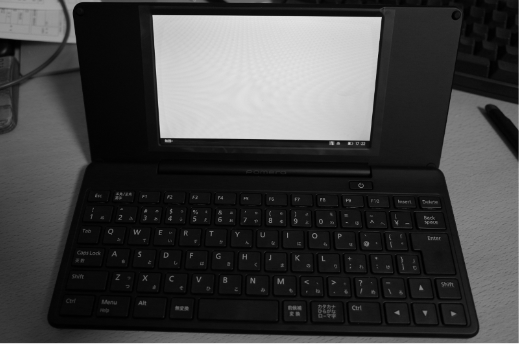
\includegraphics[scale=0.5]{image201709/dm200_gray.png}
  \end{center}
\end{figure}

筆者はサイズ感が気に入っており、MD200をPCとして使えれば良かったのに、と感じました。

DM200のアップデータが公開されたときに、配布ファイルの構成がUbuntuではないかと話題になりました。実際に筆者がアップデータファイルの内容を確認してみると、パーティション情報がそのまま結合されて保存されているように感じ、DM200はLinuxベースなOSで動作しているのではないかと予想しました。

この考察からDM200をPCのように使えるかもしれないと考え、DM200を購入してDebian化に挑戦することにしました。


\subsection{DM200の解析}

\subsubsection{シリアルコンソールの場所}

DM200を普通に利用している状態では、Linuxの糸口を得ることができませんでした。そのため中身を開けてみて、組み込み機器用のデバッグ用シリアルコンソールを探してみました。基板を探してみると、すぐに見つかりました。

\begin{figure}[h]
  \begin{center}
    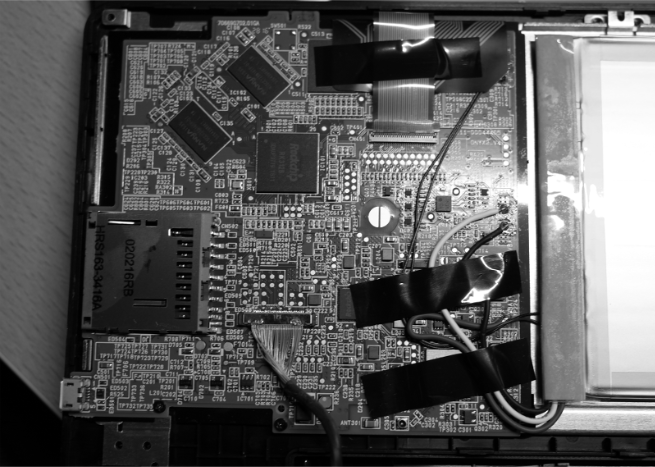
\includegraphics[scale=0.5]{image201709/dm200_board_gray.png}
  \end{center}
\end{figure}


\begin{figure}[h]
  \begin{center}
    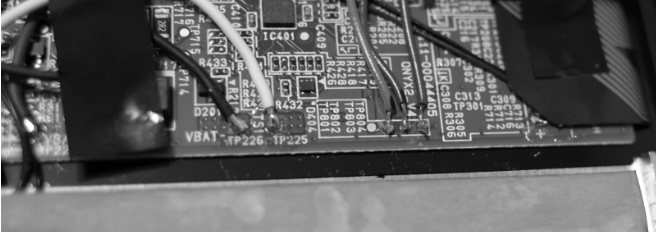
\includegraphics[scale=0.5]{image201709/dm200_board_serialconsole_gray.png}
  \end{center}
\end{figure}

\subsubsection{ソースなしでがんばってみる}

実験として、描画プログラムをとめて、シリアルコンソールから/dev/fb0に適当なデータを書き込んでみました。するとDM200の画面になにやら描画されることを確認しました。そのため、chroot環境を作ってfbtermを使えば画面に描画処理ができるのではないかと考えました。

debianのchroot環境を作成するため、qemu-debootstrapを実行します。そして、できたrootfsをSDカードへコピーします。

\begin{commandline}
# qemu-debootstrap --arch=armhf --variant=minbase
\end{commandline}

SDカードをDM200に差し込み、DM200のシリアルコンソールからSDカード上のdebian rootfsへchrootします。chroot環境のfbtermを/dev/fb0指定で起動すると、内蔵の液晶画面に描画処理を行うことができました。


しかし、動作を確認するとキーリピートが効かない、画面左上が1文字だけ表示されないなど、多くの問題も見つかりました。


chroot環境で使うよりdebianなrootfsで起動してDM200を使いたいと考え、任意のrootfsで起動する方法を模索しました。組み込み機器ではU-Bootを使っている事例が多いため、DM200もU-Bootを使っているとすれば起動処理に割り込むことで任意のrootfsを起動できると推測しました。


\subsubsection{ソースコード開示請求}

ソースコードがない状況でU-Bootであるか推測しても解析が進まないため、お客様サポートフォームへ連絡し、DVDに収めたソースコード一式を入手しました。

ソースコードを調査し、以下が判明しました。

\begin{itemize}
\item U-Bootでの割り込み処理は無効になっている
\item kernel configはそのままではLCDにコンソールは出力できないように見える
\end{itemize}

Linuxのデスクトップ環境での利用を想定したkernel configではないことから、DM200のeMMCのU-Bootとkernelを書き換える必要があると考えました。


ただ、U-Bootの置き換えは失敗すると二度と起動しなくなる可能性があり(=文鎮化)、できることなら避けたい作業です。調査を進めるとU-Bootから呼び出せるkernelは2つあるようで、片方のkernelのみを書き換えるに留めた状態でどこまでdebianが動くか試してみることにしました。

\subsection{kernelのビルド}

\subsubsection{ビルド環境の構築}

DM200向けにkernelをビルドするため、コンパイルする環境が必要になります。まずはarmhfで動作する他のボード上でkernelをセルフコンパイルしてみましたが、とても遅い状態でした。\footnote{試したのはRaspberry Pi3(\url{https://www.raspberrypi.org/products/raspberry-pi-3-model-b/})、dragonboard(\url{https://developer.qualcomm.com/hardware/dragonboard-410c})。}\footnote{ビルド処理が遅いのはストレージが遅いためかもしれません。}

そこでqemu-debootstrapで作成したarmhf環境でkernelをビルドすることにしました。

\begin{commandline}
# qemu-debootstrap --arch=armhf --variant=buildd
\end{commandline}

この環境を使ってPC上でkernelのビルドを行うと5分程度で処理が終わります。


\subsubsection{kernel configの変更とkernelのビルド}

DM200のLCD上にコンソールを出力できるようにkernelの.configファイルへ以下を追加します。

\begin{commandline}
CONFIG_VT=y
CONFIG_VT_CONSOLE=y
CONFIG_HW_CONSOLE=y
CONFIG_FRAMEBUFFER_CONSOLE=y
\end{commandline}

また、U-Bootの書き換えを行わない方針のため、kernelの起動パラメータであるCMDLINEをU-Bootの現状の指定値から変更することができません。そのため、.configに必要なCMDLINEパラメータを指定します。

\begin{commandline}
CONFIG_CMDLINE="vmalloc=496M console=tty0  \
mtdparts=rk29xxnand:0x00002000@0x00002000(uboot), \
  : (snip)
,-@0x005FA000(reserve) \
rdinit=/sbin/init root=/dev/mmcblk0p15 storagemedia=emmc \
uboot_logo=0x02000000@0x7dc00000:0x01000000 \
loader.timestamp=2016-08-29_12:54:04 \
androidboot.mode=emmc loglevel=3 rootwait"
CONFIG_CMDLINE_FORCE=y
\end{commandline}


\subsection{rootfsの作成}

rootfsがどのように作られているかは、NetBSDを使っていたときにアーキテクチャ用のパッケージを展開しただけで動作していたことを思い出し、debootstrapで作成したディレクトリツリー一式をrootfsとしてそのまま使うことにしました。

rootfsを以下のコマンドで作成しSDカードへコピーしてDM200上で動作確認したところバイナリが動作することを確認しました。\footnote{Raspberry Piのrootfsの作成も同様にdebootstrapを使っているようです。\url{https://gist.github.com/abulte/3917357}}

\begin{commandline}
# qemu-debootstrap --arch=armhf --variant=minbase --include=XX
\end{commandline}


\subsection{rootfsの引き継ぎ}

Pomeraの標準環境のinitramfsから、SDカード上のdebootstrapで作成したrootfsへswitchすることができれば、debianが起動するはずです。しかし、switch\_rootはPID 1から実行できない制約があります。そのため、initramfsも作成することにしました。

initramfsはbusyboxで作成することができます。initramfsが展開されて最初に呼ばれる/sbin/initの処理に、switch\_rootを呼び出し、SDカード上のrootfsをmountし、mountしたSDカード内にあるinitを呼び出すようなスクリプトを作成しました。

これで、DM200がdebianとしてブートするようになりました。


\subsection{Debian化後の問題点}

\subsubsection{キーリピートが効かない}

キーリピートが効かない問題は、kernelのソースコード上で無効になっていたため、kernelのソースコードを修正しました。

\begin{commandline}
arch/arm/mach-rockchip/rk312x.c
static struct tc3589x_keypad_platform_data tc35893_data = {
  .krow = 8,
  .kcol = 12,
  .debounce_period = TC_KPD_DEBOUNCE_PERIOD,
  .settle_time = TC_KPD_SETTLE_TIME,
  .irqtype = IRQF_TRIGGER_FALLING  | IRQF_ONESHOT,
  .enable_wakeup = true,
  .keymap_data    = &onxy2_keymap_data,
  .no_autorepeat  = true, ←これ。falseに変更しました。
\end{commandline}

\subsubsection{ユーザーがネットワークを使えない}

以下のkernel configが有効の場合は特定のグループ以外からsocketが使えないと調べて判明しました。kernel configのパラメータを無効に変更してkernelをビルドし直すことで解消しました。

\begin{commandline}
CONFIG_ANDROID_PARANOID_NETWORK=y ←これをnに変更
\end{commandline}


\subsubsection{PomeraのROMとDebianで時刻がずれる}

DM200のRTCから取得した時刻は、Pomera標準のファームウェアではJSTとして扱っているようです。

今回作成したDebianなrootfsではRTCをUTCとして扱う設定になっていたため、Debian側でJSTとして認識させるように変更することで解消しました。


\subsubsection{USB-OTG機能が動かない}

ハード的に見るとIDラインが結線されていないため、自動認識は無理そうでした。

ソフトで強制的に有効にすると端末が死ぬことがわかり、ドライバをいじって無理やり何とかすることで対応しました。


\subsection{今後の課題}

DM200を実用するために以下の課題を解決していく必要があると思います。

\begin{itemize}
\item 内蔵GPU(MALI400)の有効化
\item USB-OTG 有効化時に死ぬ問題の調査
\item デバイスツリーの変更を行ってみる
\item suspend処理の見直し
\item 標準の高速起動処理を流用できないか
\item 他の起動方法ができないか調べてみる
\end{itemize}

\subsection{まとめ}

DM200をハックしてみました。

組み込み機器を解析する場合にはデバッグ用のシリアルコンソールを探してみるとよいでしょう。

また、GPLなソースコードは請求して中身を見てみるといろいろ勉強になり、ソースコードがあると自分で問題を対応できて楽しいです。

qemu-debootstrapは便利なコマンドですので覚えておくとよいと思います。

%Debian / Ubuntu ユーザーミートアップ in 札幌 2017.07
\dancersection{Debian 9 Stretchのネットワークインターフェース名について}{yy\_y\_ja\_jp}
%debianmeetingresume201707-meetup-sapporo-presentation-yyoshino.tex

\subsection{ネットワークインターフェース名}
 
Debian 9 Stretchでネットワークインターフェースのデフォルトの名前が変わりました。

 \begin{itemize}
  \item Debian 8 Jessieまで
	\begin{itemize}
	 \item 有線LANインターフェース: eth0, eth1, ...
	 \item 無線LANインターフェース: wlan0, wlan1, ...
	\end{itemize}
  \item Debian 9 Stretchから
	\begin{itemize}
	 \item 有線LANインターフェース: enp0s1 など、ハードウェア構成に
	       より異なる
	 \item 無線LANインターフェース: wlp1s0 など、ハードウェア構成に
	       より異なる
	\end{itemize} 
 \end{itemize}

\subsection{Jessie からアップグレードしたときは}

 \begin{itemize}
  \item 今まで使っていたインターフェースの名前は変わりません
  \item 今後新たに使うインターフェースは新しい名前の形式になります -- 新
	しいUSB NICを差したときなど
 \end{itemize}
 \texttt{/usr/share/doc/udev/README.Debian.gz}によると
 Debian 10 Busterでは昔の方式はサポートされないと言ってるので、新しい名前に移行したほうが
 よいかもしれません。

\subsection{なぜデフォルトの名前が変わったのか}
今までの名前の変え方だとうまくいかないことがあったため、今回改定すること
になりました。

今までdmesgなどで、\texttt{eth0: renamed from eth1} などといったメッセー
ジを見たことがある方もいると思います。
もともと、ネットワークインターフェースの名前はOSの起動中に変えている(こ
とがある)ものなのです。

\subsection{なぜ名前を変えているのか}
 \begin{itemize}
  \item Linux カーネルはネットワークインターフェースを認識するたびに名前を付
	けている eth0, eth1, ...
  \item 認識する順番は保証されない\\
	⇒ ネットワークインターフェースが複数あるときは、同じインター
	フェースが起動するたびに別の名前になることがある\\
	⇒ カーネルで認識されたらユーザーランド側で名前を修正することに
	した
 \end{itemize}

\subsection{名前の変え方 -- Jessieまで}
 udevパッケージの

 \texttt{/lib/udev/rules.d/75-persistent-net-generator.rules} と
 \texttt{/lib/udev/write\_net\_rules}\\
 (Stretch にはもう存在しません!)が名前を変えていました。

 知らないインターフェースが現れたら次のように動作します。
 \begin{enumerate}
  \item 空いている次の番号の名前を探す: eth1 など
  \item 「そのインターフェースが現れたらその名前に変える」というudevルールを\\
	\texttt{/etc/udev/rules.d/70-persistent-net.rules} という設定ファ
	イルに
	書き込む
  \item その名前に変える
 \end{enumerate}

 Stretchではこれらのプログラムは無くなったため、
\texttt{/etc/udev/rules.d/70-persistent-net.rules} ファイルが今後自動で書き換
 わることはありません。


\subsection{名前の変え方 -- Stretchから}
 udevパッケージの
 \texttt{/lib/udev/rules.d/75-net-description.rules}、
 udevの\texttt{net\_id}ビルトイン、
 \texttt{/lib/udev/rules.d/80-net-setup-link.rules}、
 \texttt{net\_setup\_link}ビルトイン、\\
 \texttt{/lib/systemd/network/99-default.link} などが名前を変えています。

 知らないインターフェースが現れたら次のように動作します。
 \begin{enumerate}
  \item そのインターフェースを特定する情報(ハードウェア配置、MACアド
	レス、ユーザー設定ファイルなど)を取得する
  \item その情報に基づいて名前を決める: PCIバス0のスロット1に差さって
	いるとき enp0s1 など\\
	ただしUSB NICの場合は、USBの差す位置で名前が変わって
	ほしくないのでMACアドレスベースの名前にする設定になっている(\texttt{/lib/udev/rules.d/73-usb-net-by-mac.rules}): enxaabbccxxyyzz など
 \end{enumerate}


\subsection{名前の変え方 -- (参考)一時期のUbuntu}
 Debianにはないですが、Ubuntuはbiosdevnameパッケージで名前を決めている時期が
 ありました。なお、現在のインターフェース名とは互換性がありません。

 \begin{itemize}
  \item インターフェース名: em0, p1p0 など
  \item 後発のudev net\_idはさらに別の名前形式にした。そのため互換性がな
	い
 \end{itemize}


\subsection[containsverbatim]{移行するには}

 \begin{enumerate}%
  \item どんな名前になるか調べる。eth0なら\\
	\texttt{udevadm test-builtin net\_id /sys/class/net/eth0}
\begin{commandline}
# udevadm test-builtin net_id /sys/class/net/eth0
calling: test-builtin
(略)
Parsed configuration file /lib/systemd/network/99-default.link
Created link configuration context.
ID_NET_NAME_MAC=enx000d0bxxyyzz
ID_OUI_FROM_DATABASE=BUFFALO.INC
ID_NET_NAME_PATH=enp0s20u2
Unload module index
Unloaded link configuration context.
\end{commandline}
	\texttt{ID\_NET\_NAME\_*}のうち、順に
	\texttt{ONBOARD}、\texttt{SLOT}、
	\texttt{PATH}がもしあればそれが使われる\\
(\texttt{/lib/systemd/network/99-default.link})、ただしUSB NICは\texttt{MAC}が使われる
  \item 今までの名前を使っている設定ファイルを置き換える
  \item \texttt{/etc/udev/rules.d/70-persistent-net.rules} を消
	すかどこかに移動する
  \item 再起動
 \end{enumerate}


\subsection[containsverbatim]{移行せず、名前を変えさせないには}
 もともとインターフェースが1つしかない、eth0, wlan0しかなかったのに変え
 てほしくないときなどは、
 いくつか方法があります。
\begin{itemize}
 \item 空っぽの設定ファイルを\texttt{/etc}に置いて上書きする\\
       \verb|ln -s /dev/null /etc/systemd/network/99-default.link|
 \item カーネルコマンドライン引数に\texttt{net.ifnames=0}を追加\\
       /etc/default/grub に書いて update-grub を実行
\end{itemize}

 もちろんこうするとカーネルが決めた名前そのままになるので、インターフェースが複数
 あったらうまくいかないことが起きるでしょう。


\subsection[containsverbatim]{名前を自分で設定するには}
\begin{itemize}
 \item \texttt{net\_setup\_link}のユーザー設定ファイル \texttt{/etc/systemd/network/*.link}
       を作る(systemd.link(5))\\
       例えばMACアドレス aa:bb:cc:xx:yy:zz のインターフェースを ethernet1 という名前にしたいなら
\begin{commandline}
[Match]
MACAddress=aa:bb:cc:xx:yy:zz
[Link]
Name=ethernet1
\end{commandline}
ただし、USB NICの名前を設定するには\\
       \verb|ln -s /dev/null /etc/udev/rules.d/73-usb-net-by-mac.rules|\\
       が必要
 \item udevルールファイル \texttt{/etc/udev/rules.d/*.rules} を作
       る(udev(7))\\
       Jessieまで自動で書き込まれてきた 
       \texttt{/etc/udev/rules.d/70-persistent-net.rules} ファイルに同
       じように追加する、など
\end{itemize}


\subsection[containsverbatim]{うまくいかないときは}
 udev をデバッグするしかないです。
\begin{itemize}
 \item 書いた\texttt{*.link}が期待通りに動くか見るには \texttt{net\_setup\_link}ビルトインを試す:\\
       \verb|udevadm test-builtin net_setup_link /sys/class/net/eth0|
 \item udevをdebugモードで起動する
\begin{commandline}
# invoke-rc.d udev stop
# /lib/systemd/systemd-udevd --debug
\end{commandline}
 \item マシン起動時のudevをdebugモードにする\\
       /etc/udev/udev.conf を \verb|udev_log="debug"| にして
       \verb|dpkg-reconfigure linux-image-`uname -r`|
       して再起動
\end{itemize}

 名前変更に失敗してカーネルが決めた名前のままになっていることがあったり
 します...
 見つけたらバグレポートしたほうがよいかもしれません。


\subsection{まとめ}
\begin{itemize}
 \item udevが変わり、Debian 9 Stretch からはネットワークインターフェースが新しい名前の
       形式になった
 \item 新しいインターフェースは新しい名前になる
 \item Jessie からアップグレードした場合は直ちに影響はないが、変えたほう
       がいいらしい
 \item 移行前に新しい名前を見るには\\
 \texttt{udevadm test-builtin net\_id /sys/class/net/<今の名前>}\\
 などが使える
 \item 名前付け替えを一切したくないときは \texttt{/etc} で
       \texttt{99-default.link}を上書き設定するとよい
 \item 自分で名前を付けたいときは
       \texttt{/etc/systemd/network/*.link} を作る、
       または昔ながらの udev ルール
       \texttt{/etc/udev/rules.d/*.rules} を作る
 \item うまく行かないときは udev をデバッグする。
       名前変更に失敗して元の名前のままになっていることがある
\end{itemize}



\subsection{参考文献}
\begin{itemize}
 \item PredictableNetworkInterfaceNames\\
      \url{http://www.freedesktop.org/wiki/Software/systemd/PredictableNetworkInterfaceNames/}
 \item systemd ソースパッケージ \verb|src/udev/udev-builtin-net_id.c|
 \item udev パッケージ \verb|/usr/share/doc/udev/README.Debian.gz|, man
       ページ \verb|systemd.link(5)|, \verb|udev(7)|
 \item biosdevname パッケージ(Ubuntu)
\end{itemize}


%XXX
%

%201708 kansai
% ---------------------------------------------------
\dancersection{Debian Stretchのインプットメソッドの現状}{あわしろいくや}

\subsection{はじめに}

去る6月17日にリリースされたDebian GNU/Linux 9.0 StretchのGNOME版を(仮想マシンに)インストールしてみましたが、日本語入力が難解であるという印象を持ちました。私はUbuntuでインプットメソッド関連をごそごそしている経験があり、その知識を元にDebian 9.0の各デスクトップ環境でスムーズにインプットメソッドを使用する方法を探っていきたいと思います。

なお、今後の提案等も含まれていますが、私自身は全く手を動かせないということをあらかじめご了承ください。

\subsection{パッケージがインストールされる仕組み}

Debian Installerでインストールすると、選択した項目に応じて日本語関連のパッケージもインストールされます。パッケージの選択はtasksの仕組みを使用しています。

\subsubsection{task-japanese}

日本語を選択するとインストールされます。
実際にインストールされるパッケージは次のとおりです。
\begin{commandline}
  manpages-ja, lv, fbterm, unifont, nkf, manpages-ja-dev
\end{commandline}

\subsubsection{task-japanese-desktop}

日本語とデスクトップ環境を選択するとインストールされます。実際にインストールされるパッケージは次のとおりです。
\begin{commandline}
  firefox-esr-l10n-ja | firefox-l10n-ja, fonts-vlgothic, fonts-ipafont,
  uim, uim-anthy, uim-mozc, mozc-utils-gui, anthy, libreoffice-l10n-ja, libreoffice-help-ja, poppler-data
\end{commandline}

\subsubsection{task-japanese-gnome-desktop}

日本語とGNOMEデスクトップ環境を選択するとインストールされます。実際にインストールされるパッケージは次のとおりです。

\begin{commandline}
  uim-applet-gnome, icedove, icedove-l10n-ja
\end{commandline}

おや、icedoveパッケージはthunderbirdに名前が戻りましたね\ldots{}\ldots{}。

\subsubsection{task-japanese-kde-desktop}

日本語とKDE
SCを選択するとインストールされます。最近はKDEデスクトップ環境はKDE SC
(Software
Compilation)と呼んでいます。実際にインストールされるパッケージは次のとおりです。

\begin{commandline}
  kde-l10n-ja, plasma-widget-uim
\end{commandline}

tasksにあるインプットメソッド(uim)を自動起動するためには\texttt{im-config}パッケージが必要ですが、これは\texttt{libuim-data}パッケージに引っ張られてインストールされます。

\subsection{自動実行の仕組み}

前述のとおり、インプットメソッドの自動起動には\texttt{im-config}パッケージが使われています。これは各インプットメソッドの情報がまとめられており、IBusとFcitxとuimでは次のようになっています。

\begin{itemize}
\item /usr/share/im-config/
  \begin{itemize}
  \item
    data/21\_ibus*
  \item
    data/22\_fcitx*
  \item
    data/24\_uim*
  \end{itemize}
\end{itemize}

これは番号が若いほうが優先度が高くなっています。すなわち、デフォルトではIBusとFcitxとuimが同時にインストールされている場合はIBusが優先して起動されます。

もちろん手動での設定も可能になっており、前述の3つが同時にインストールされている場合にFcitxを優先して起動するためには次のコマンドを実行します。

\begin{commandline}
  $ im-config -n fcitx
\end{commandline}
% $
GUIの設定ツールもあります。

\subsection{GNOME Shellの場合}
\begin{wrapfigure}{r}{5.5cm}
    \begin{center}
        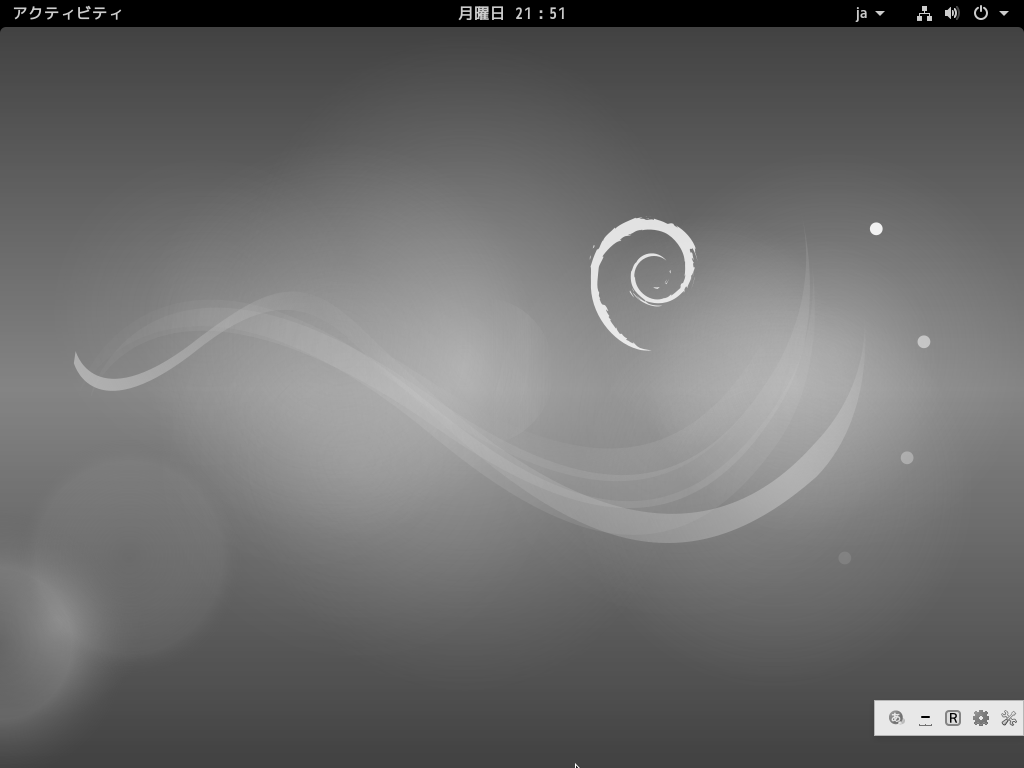
\includegraphics[width=5cm]{image201708/gnome-uim-toolbar-gtk3_gray.png}
        \caption{GNOME Shellでuim-toolbar-gtk3を表示したところ}
    \end{center}
\end{wrapfigure}
では、ここから各デスクトップ環境ごとの挙動を見ていきます。

インストール時にGNOMEを選択し、最初にログインすると英語キーボードと(接続されている場合)日本語キーボードを認識しています。

GNOME ShellはIBusと統合されており、現状IBusと共に使われることが意図されています。しかし、Debianでは前述のとおりデフォルトのインプットメソッドはuimなので、統合機能は全く使用することができません。

半角/全角キーを押すと日本語が入力できるようになるため、uimが正常に動作していることはわかります。しかし、ステータスは全くわかりません。

psコマンドで確認するとuim-toolbarというプロセスがいます。lsコマンドで確認するとalternativesで管理されていることがわかり、実体は/usr/bin/uim-toolbar-gtk3-systrayになっています。

現在のGNOME Shellにもレガシートレイとしてuim-toolbar-gtk3-systrayを表示する機能がありますが、なぜか表示されません。gnome-shell-extension-top-icons-plusをインストールして有効にすれば表示されるはずですが、やはり表示されません。uim-toolbar-gtk3-systrayの起動するタイミングが早すぎるのが問題と思われ、手動で起動すれば表示されます。

現実的にはalternativesでuim-toolbar-gtk3に切り替え、ツールバーを表示するのがいいでしょう。

\subsection{KDE Plasmaの場合}
\begin{wrapfigure}{r}{5.5cm}
    \begin{center}
        
\includegraphics[width=5cm]{image201708/kde-uim-toolbar-qt5_gray.png}
        \caption{KDE Plasmaでuim-toolbar-qt5を表示したところ}
    \end{center}
\end{wrapfigure}

インストール時にKDEを選択し、最初にログインすると右下のトレイに妙にカラフルなアイコンがありますが、これはおそらくuim-toolbar(実体はuim-toolbar-gtk3-systray)が1つのアイコンの大きさに圧縮されているものと思われます。uimにはuim-toolbar-qt4/5があるので、これを選択するのがいいでしょう。

前述のとおりplasma-widget-uimがインストールされているので、これを有効にしたいところですが、追加できるウィジェットに表示されません。おそらく現状の実装がKDE
Plasma
4.x対応で5.xに対応していないのが原因と思われます。確認したところDebian
Jessieでは追加できるウィジェットに表示されていました。

\subsection{Cinnamonの場合}
\begin{wrapfigure}{r}{5.5cm}
    \begin{center}
        
\includegraphics[width=5cm]{image201708/cinnamon_gray.png}
        \caption{Cinnamonのログイン直後の状態}
    \end{center}
\end{wrapfigure}

インストール時にCinnamonを選択し、最初にログインすると右下のトレイにアイコンが表示されます。一見このままでもよさそうですが、入力が直接入力なのかひらがな入力なのかカタカナ入力なのかそれ以外なのか極めてわかりにくいです。よってuim-toolbar-gtk3を使用するといいでしょう。

\subsection{Xfceの場合}
\begin{wrapfigure}{r}{5.5cm}
    \begin{center}
        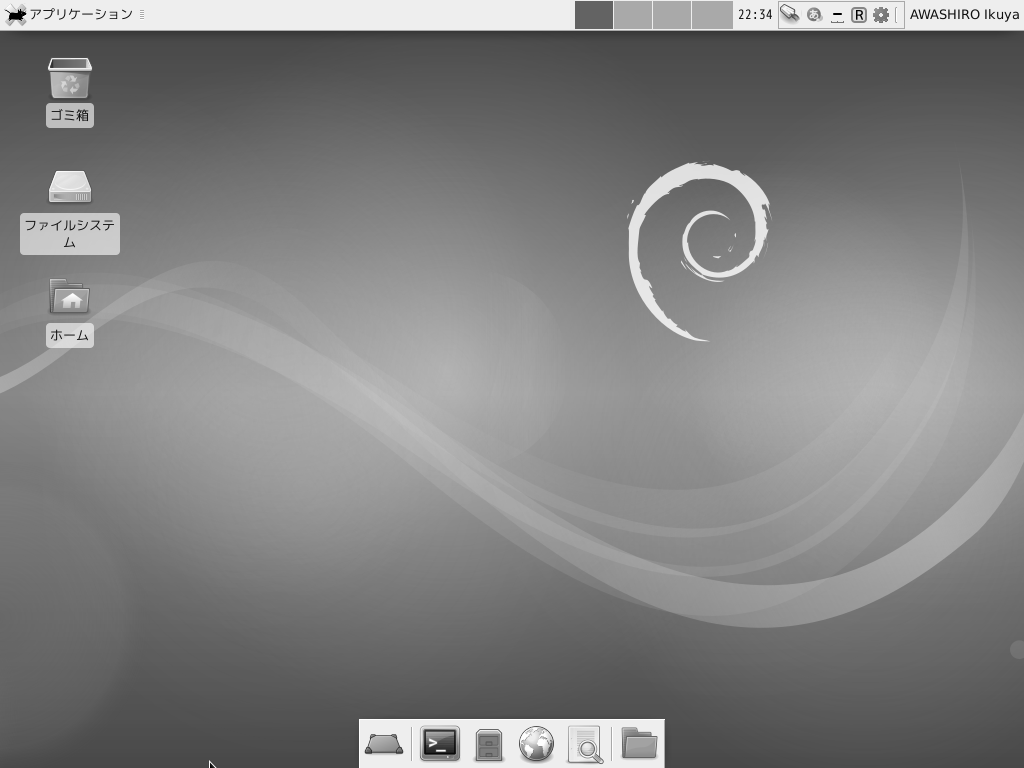
\includegraphics[width=5cm]{image201708/xfce_gray.png}
        \caption{Xfceのログイン直後の状態}
    \end{center}
\end{wrapfigure}

インストール時にXfceを選択し、最初にログインすると右上にuimのステータスがすべて表示されています。今回は紹介しませんが、MATEやLXDEを選択してもこのように表示されると思われます。理想的ではありますが、システムトレイのツールキットがGTK+
2か3かで表示方法を分けているようであり、Xfceでは前者なのでいずれ対応しなくなると思われます。sidのMATEはすでにGTK+
3でビルドされているため、一つ分のトレイアイコンしか表示されないはずです。

\clearpage

\subsection{uim-mozcの問題}

uim-mozcを使用すると、Mozcの各種ツール(mozc\_tool)が起動しません\footnote{https://bugs.debian.org/cgi-bin/bugreport.cgi?bug=700307}。正確にはprotobufの問題\footnote{https://bugs.debian.org/cgi-bin/bugreport.cgi?bug=721791}ですが、もう何年も未解決です。IBusやFcitxにはこのような問題がないため、uim-mozcを避けることができるのであれば避けたほうがいいでしょう。

\subsection{短期的な修正の提案}
\begin{wrapfigure}{r}{5.5cm}
    \begin{center}
        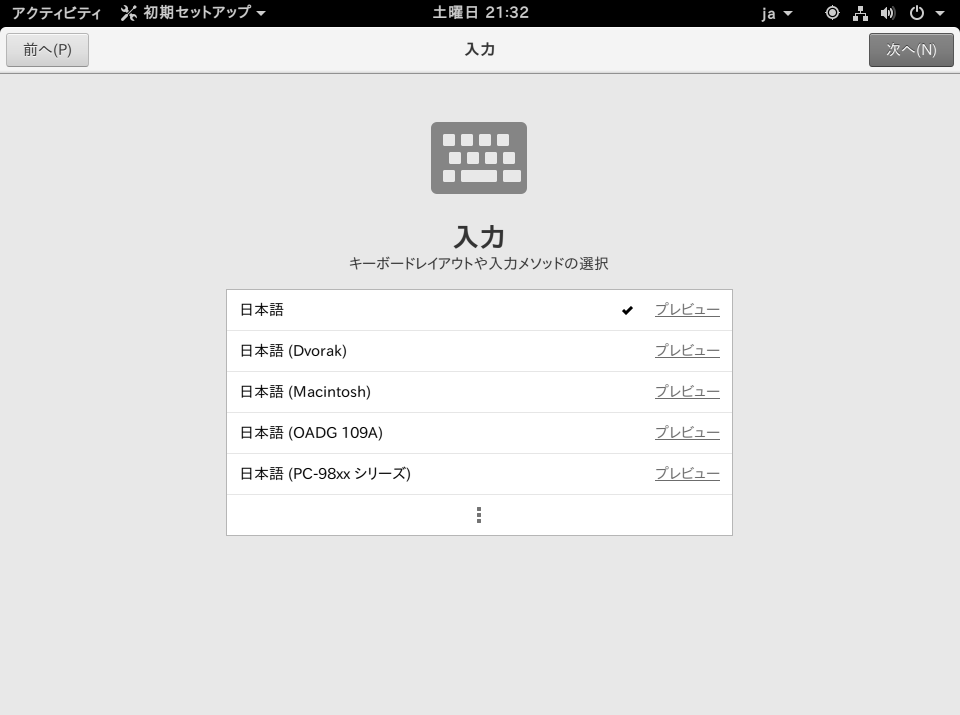
\includegraphics[width=5cm]{image201708/gnome-initial-setup_gray.png}
        \caption{初期セットアップ(Ubuntu GNOME 17.04のもの)}
    \end{center}
\end{wrapfigure}
以上の現状を鑑みるに、インストールする人が多そうなGNOMEが特に影響が大きいので、短期的にどうにかできるものであればしたほうがいいのかもしれません。GNOMEの場合は専用のタスクがあるので、これだけをいじればなんとかなるということもあります。

GNOMEは現状IBusで使用することしか考えられていないため、IBus一式と初期セットアップ(gnome-initial-setup)をtask-japanese-gnome-desktopに追加すれば、おおむね問題が解決します。初期セットアップは初回ログイン時に各種設定を行いますが、その中にキーボードやインプットメソッド(GNOMEでは同様に扱われる)の設定も含まれるため、設定の難易度が大幅に低下します。

\subsection{長期的な修正の提案}

長期的には、uimからIBusに移行するのがよさそうに思います。uimのメンテナンスは現状特定の個人に負荷が集中していますが、IBusであればある程度負荷が分散されているというのが大きな理由です。特に各種ツールキットやデスクトップ環境向けの対応を考えなくてもいいのが楽です。技術的には概ねこれまで挙げてきた問題が解決されますが、uimでは問題とならなかったことが問題となり得ます。具体的には愛用者が多いと思われるSKKの実装であるibus-skkやそのバックエンドのlibskkが現在メンテナーがいないこと、fbtermで使用するibus-fbtermがパッケージになっておらず、またなったとしてもどの程度実用的なのか疑問符がつくことです。

もちろんFcitxも選択肢に入ってきますが、現状のFcitxはWaylandに非対応でかつツールキットはQt
4であり、現在最新バージョンであるFcitx5の開発中ですが、Fcitx5のリリースが早いかQt
4の削除が早いかは誰にもわかりません。ちなみに中国語(簡体字)ではFcitxが使用されているため、このリソースに乗っかれるというメリットはあります。

uimを使い続けるのであれば、uim-toolbarの切り替えをalternativesでやるのではなく、環境変数を使用してデスクトップ環境に応じてより適切な選択をするのがいいと思います。ただしQt/KDE
Plasma 5対応をより進め、また開発が進んでいるGTK+
4にも対応していくのは、かなりの労力が必要なことでしょう。

% ---------------------------------------------------

%-------------------------------------------------------------------------------
\dancersection{Rethinking Debian release}{Yamane Hideki}
%-------------------------------------------------------------------------------

この発表は議論のたたき台としてDebian勉強会で発表されたもので、決定事項等ではありません。
この資料は勉強会での英語の発表資料\footnote{https://wiki.debian.org/HidekiYamane/material?action=AttachFile\&do=view\&target=Rethinking-debian-release.pdf}から編者(吉田)がコンバートしたものです。
%元資料 https://wiki.debian.org/HidekiYamane/material?action=AttachFile&do=view&target=Rethinking-debian-release.pdf

\subsection{Why rethink release?}
\begin{itemize}
%\item“Debian is old”
%\item“Debian (stable) is old”
\item“Debian (stable) is old (for our usage)”
\item“Some packages are still old and buggy,but no update”
\end{itemize}

\subsection{Current Release Migration}
\begin{itemize}
 \item Unstable → Testing
  \begin{itemize}
   \item Based on urgency (high,medium,low)
    \begin{itemize}
     \item Blocked by Release Critical bug
    \end{itemize}
  \end{itemize}
 \item Testing → Stable
  \begin{itemize}
   \item (Looong) Freeze and release
  \end{itemize}
\end{itemize}

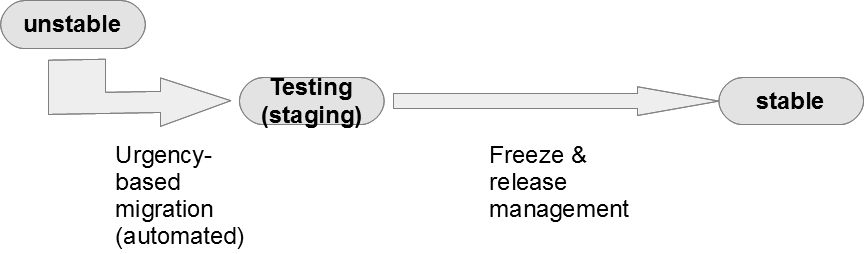
\includegraphics[width=\linewidth]{image201711-tokyo/Rethinking-debian-release-p3_gray.png}

\subsection{Stable release management  = many-legged-race}
\noindent
Push release management causes
\\
“many(60,000-70,000 Packages)-legged-race”
\\
%Its result...
%Like this...
%https://www.youtube.com/watch?v=Rwqvx99Gz2U

\subsection{Another Problem:Is that package tested, really?}

\begin{itemize}
 \item Who tests it?
  \begin{itemize}
   \item Sometimes "Passive test" doesn't work well
  \end{itemize}
 \item Code never matures
  \begin{itemize}
   \item Code != Wine / Whiskey
   \item But time makes features to rot...
  \end{itemize}
\end{itemize}

\subsection{Worst scenario}
\begin{itemize}
 \item Upload to unstable
  \begin{itemize}
   \item → no one cares it
   \item → no bugs filed
   \item → migrate to testing
   \item → release stable
   \item → found bugs in stable, but leave it...
  (since put not tiny changes to stable is not easy task…)
   \item → bad user experience
   \item → bad reputation
   \item → less user
   \item → less developer...
  \end{itemize}
\end{itemize}
   
\subsection{Answer (1):“Active” migration}

\begin{itemize}
 \item Same as other distros
  \begin{itemize}
   \item  Gentoo: mask (package flag)
   \item  Fedora: bohdi (voting system)
   \item  openSUSE: openQA (automated test)
  \end{itemize}
 \item "pull" migration system via vote by users \& maintainers
  \begin{itemize}
   \item “Package quality” is guaranteed by safety harness (pipeline)
  \end{itemize}
 \item It ensure "it works" by someone, at least
\end{itemize}

\subsection{Pull is better than push}
\begin{itemize}
 \item “Push” Testing to stable migration
  \begin{itemize}
    \item Thousands changes in one time
    \item {itemize}Handled by few release managers
     \begin{itemize}
      \item = capacity overflow → burnout...
     \end{itemize}
  \end{itemize}
\end{itemize}

\begin{itemize}
 \item “Pull” migration
  \begin{itemize}
    \item Several changes in one time
    \item Handled by hundreds advanced users \& maintainers
  \end{itemize}
\end{itemize}

\subsection{Answer (2):New distribution}
\noindent
Why we need "new distribution"?
\\
Average users never use unstable or testing, they use "released" one (= stable)
\\
“Innovators theory” (by Everett M. Rogers)
\\
\begin{itemize}
 \item Innovators			: 	 2.5%	(unstable)
 \item Early Adopters		:		13.5%	(testing)
 \item Early Majority		:		34.0%
 \item Late Majority		: 	34.0%	(stable)
 \item Laggards			: 		16.0%	(oldstable)
\end{itemize}

“Fresh” distribution
\begin{itemize}
 \item Innovators		: 	 2.5%		(unstable)
 \item Early Adopters	:		13.5%		(testing)
 \item Early Majority	:		34.0%		“Fresh”
 \item Late Majority	: 	34.0%		(stable)
 \item Laggards			: 	16.0 %		(oldstable)
\end{itemize}
We can get more users! (100 / 66 = 150%)
\\
\subsection{Positioning}

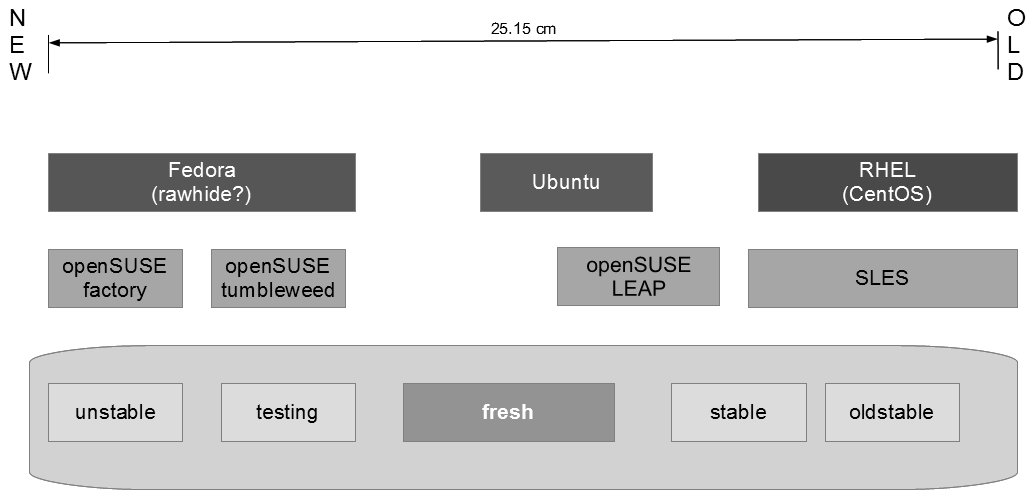
\includegraphics[width=\linewidth]{image201711-tokyo/Rethinking-debian-release-p13_gray.png}

\subsection{Fresh?}
\noindent
Borrow name from LibO :)
\\
Target: Average users (Early Majority)
\\
Release every one or two week
\begin{itemize}
 \item Rolling release
 \item Predictable scheduled release
\end{itemize}
Pull change sets
\begin{itemize}
 \item Sustainable deploy
 \item Ensure changes, not break anything
\end{itemize}
Not push changes into stable directly
\\
Why new “fresh” distribution?
\begin{itemize}
 \item Users expect stable as stable (≒ not changed so much)
 \item We afraid to break stable release
\end{itemize}
\subsection{Migration cycle time}
\noindent
Traditional migration
\\
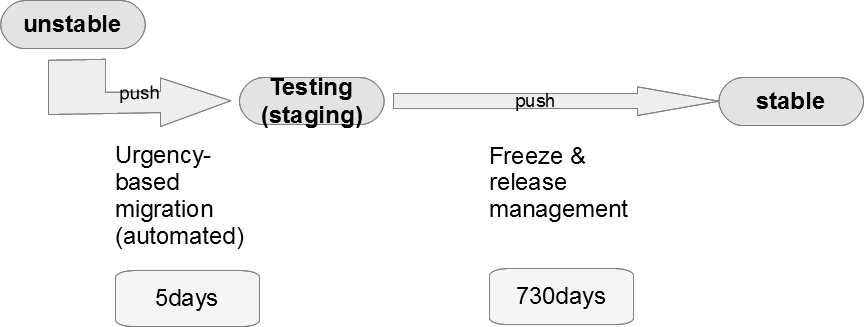
\includegraphics[width=\linewidth]{image201711-tokyo/Rethinking-debian-release-p16_gray.png}

\noindent
Add “Fresh” distribution\\
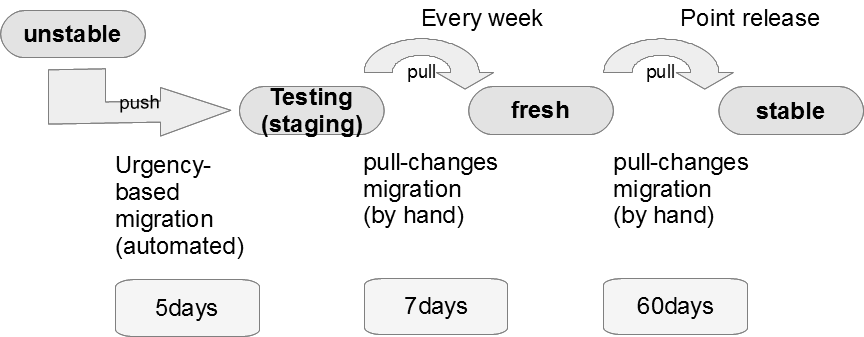
\includegraphics[width=\linewidth]{image201711-tokyo/Rethinking-debian-release-p17_gray.png}

\subsection{Shorten cycle time}
\noindent
Before		: 730 days (minimum 180days)
\\
After		: 12 days
\\
15-60 times faster delivery!
\\
Maximize added-value

\subsection{Change the rule!}
\noindent
There was a reason to make rules
\begin{itemize}
 \item Unstable - Testing - Stable
 \item Long freeze term and release
\end{itemize}
But situation has changed, then rules should be changed, too. Because its rule becomes bottlenec

\subsection{Faster release introduce more bugs?}
\noindent
Q: It may introduce more bugs!\\
A: “test early and fail fast” on fresh stage, but less bugs in stable since more test users watch it.\\
Testers
\begin{itemize}
 \item Previous	: 2.5 + 13.5 = 16.0
 \item Fresh		: 2.5 + 13.5 + 34.0 = 50.0 → 300%
\end{itemize}
\subsection{“Fresh”: Pros \& Cons}
\noindent
Pros)
\begin{itemize}
 \item 150% users, 300% testers
 \item 60 times faster release
 \item Same cadence, its release date \& changes are predictable
 \item Changes in each release are small, users can bite it (No Big Bang release)
  \begin{itemize}
   \item Less freeze term for next release
   \item Not need to hassle to make huge release note
   \item Moe "real acceptance test" by real users for next stable release
  \end{itemize}
\end{itemize}
Cons)
\begin{itemize}
 \item It just costs
 \item Infrastructure change
 \item Docs \& website update
 \item More release manager \& publicity work
 \item Prepare security fix (but delta with unstable is small, right?)
  \begin{itemize}
   \item maybe it reduce backport effort in stable
  \end{itemize}
\end{itemize}
\subsection{Metrics?}
\noindent
More testers / More users
\begin{itemize}
 \item BTS number
 \item RC in stable / bugs in stable
 \item Download number
\end{itemize}

%-------------------------------------------------------------------------------
\dancersection{Debian Trivia Quiz}{}
%-------------------------------------------------------------------------------

ところで、みなさん Debian 関連の話題においついていますか?Debian関連の話
題はメーリングリストをよんでいると追跡できます。ただよんでいるだけではは
りあいがないので、理解度のテストをします。特に一人だけでは意味がわからな
いところもあるかも知れません。みんなで一緒に読んでみましょう。

今回の出題範囲は\url{debian-devel-announce@lists.debian.org} や \url{debian-devel@lists.debian.org}に投稿された
内容とDebian Project Newsからです。

\small
\begin{multicols}{2}
%; whizzy-master ../debianmeetingresume201311.tex
% $B0J>e$N@_Dj$r$7$F$$$k$?$a!"$3$N%U%!%$%k$G(B M-x whizzytex $B$9$k$H!"(Bwhizzytex$B$,MxMQ$G$-$^$9!#(B
%

\santaku
{quiz}
{answer A}
{answer B}
{answer C}
{B}
{desc}

\end{multicols}
\normalsize

%for less page
%\printindex

\newpage

\begin{center}
本資料のライセンスについて
\end{center}

\begin{fontsize}{6}{6}

本資料はフリー・ソフトウェアです。あなたは、Free Software
Foundation が公表したGNU GENERAL PUBLIC LICENSEの "バージョン2"もしくはそれ以降
が定める条項に従って本プログラムを再頒布または変更することができ
ます。

本プログラムは有用とは思いますが、頒布にあたっては、市場性及び特
定目的適合性についての暗黙の保証を含めて、いかなる保証も行ないま
せん。詳細についてはGNU GENERAL PUBLIC LICENSE をお読みください。

\end{fontsize}

\begin{center}
ソースコードについて
\end{center}

本資料のソースコードは Git を使って\url{git://anonscm.debian.org/tokyodebian/monthly-report.git}
からダウンロードできます。以下に方法を示します。

\begin{commandline}
$ git clone git://anonscm.debian.org/tokyodebian/monthly-report.git
\end{commandline}
%$

\begin{multicols}{2}
 \begin{fontsize}{6}{6}
 \begin{verbatim}
            GNU GENERAL PUBLIC LICENSE
               Version 2, June 1991

 Copyright (C) 1989, 1991 Free Software Foundation, Inc.
    51 Franklin St, Fifth Floor, Boston, MA  02110-1301  USA
 Everyone is permitted to copy and distribute verbatim copies
 of this license document, but changing it is not allowed.

                Preamble

  The licenses for most software are designed to take away your
freedom to share and change it.  By contrast, the GNU General Public
License is intended to guarantee your freedom to share and change free
software--to make sure the software is free for all its users.  This
General Public License applies to most of the Free Software
Foundation's software and to any other program whose authors commit to
using it.  (Some other Free Software Foundation software is covered by
the GNU Library General Public License instead.)  You can apply it to
your programs, too.

  When we speak of free software, we are referring to freedom, not
price.  Our General Public Licenses are designed to make sure that you
have the freedom to distribute copies of free software (and charge for
this service if you wish), that you receive source code or can get it
if you want it, that you can change the software or use pieces of it
in new free programs; and that you know you can do these things.

  To protect your rights, we need to make restrictions that forbid
anyone to deny you these rights or to ask you to surrender the rights.
These restrictions translate to certain responsibilities for you if you
distribute copies of the software, or if you modify it.

  For example, if you distribute copies of such a program, whether
gratis or for a fee, you must give the recipients all the rights that
you have.  You must make sure that they, too, receive or can get the
source code.  And you must show them these terms so they know their
rights.

  We protect your rights with two steps: (1) copyright the software, and
(2) offer you this license which gives you legal permission to copy,
distribute and/or modify the software.

  Also, for each author's protection and ours, we want to make certain
that everyone understands that there is no warranty for this free
software.  If the software is modified by someone else and passed on, we
want its recipients to know that what they have is not the original, so
that any problems introduced by others will not reflect on the original
authors' reputations.

  Finally, any free program is threatened constantly by software
patents.  We wish to avoid the danger that redistributors of a free
program will individually obtain patent licenses, in effect making the
program proprietary.  To prevent this, we have made it clear that any
patent must be licensed for everyone's free use or not licensed at all.

  The precise terms and conditions for copying, distribution and
modification follow.

            GNU GENERAL PUBLIC LICENSE
   TERMS AND CONDITIONS FOR COPYING, DISTRIBUTION AND MODIFICATION

  0. This License applies to any program or other work which contains
a notice placed by the copyright holder saying it may be distributed
under the terms of this General Public License.  The "Program", below,
refers to any such program or work, and a "work based on the Program"
means either the Program or any derivative work under copyright law:
that is to say, a work containing the Program or a portion of it,
either verbatim or with modifications and/or translated into another
language.  (Hereinafter, translation is included without limitation in
the term "modification".)  Each licensee is addressed as "you".

Activities other than copying, distribution and modification are not
covered by this License; they are outside its scope.  The act of
running the Program is not restricted, and the output from the Program
is covered only if its contents constitute a work based on the
Program (independent of having been made by running the Program).
Whether that is true depends on what the Program does.

  1. You may copy and distribute verbatim copies of the Program's
source code as you receive it, in any medium, provided that you
conspicuously and appropriately publish on each copy an appropriate
copyright notice and disclaimer of warranty; keep intact all the
notices that refer to this License and to the absence of any warranty;
and give any other recipients of the Program a copy of this License
along with the Program.

You may charge a fee for the physical act of transferring a copy, and
you may at your option offer warranty protection in exchange for a fee.

  2. You may modify your copy or copies of the Program or any portion
of it, thus forming a work based on the Program, and copy and
distribute such modifications or work under the terms of Section 1
above, provided that you also meet all of these conditions:

    a) You must cause the modified files to carry prominent notices
    stating that you changed the files and the date of any change.

    b) You must cause any work that you distribute or publish, that in
    whole or in part contains or is derived from the Program or any
    part thereof, to be licensed as a whole at no charge to all third
    parties under the terms of this License.

    c) If the modified program normally reads commands interactively
    when run, you must cause it, when started running for such
    interactive use in the most ordinary way, to print or display an
    announcement including an appropriate copyright notice and a
    notice that there is no warranty (or else, saying that you provide
    a warranty) and that users may redistribute the program under
    these conditions, and telling the user how to view a copy of this
    License.  (Exception: if the Program itself is interactive but
    does not normally print such an announcement, your work based on
    the Program is not required to print an announcement.)

These requirements apply to the modified work as a whole.  If
identifiable sections of that work are not derived from the Program,
and can be reasonably considered independent and separate works in
themselves, then this License, and its terms, do not apply to those
sections when you distribute them as separate works.  But when you
distribute the same sections as part of a whole which is a work based
on the Program, the distribution of the whole must be on the terms of
this License, whose permissions for other licensees extend to the
entire whole, and thus to each and every part regardless of who wrote it.

Thus, it is not the intent of this section to claim rights or contest
your rights to work written entirely by you; rather, the intent is to
exercise the right to control the distribution of derivative or
collective works based on the Program.

In addition, mere aggregation of another work not based on the Program
with the Program (or with a work based on the Program) on a volume of
a storage or distribution medium does not bring the other work under
the scope of this License.

  3. You may copy and distribute the Program (or a work based on it,
under Section 2) in object code or executable form under the terms of
Sections 1 and 2 above provided that you also do one of the following:

    a) Accompany it with the complete corresponding machine-readable
    source code, which must be distributed under the terms of Sections
    1 and 2 above on a medium customarily used for software interchange; or,

    b) Accompany it with a written offer, valid for at least three
    years, to give any third party, for a charge no more than your
    cost of physically performing source distribution, a complete
    machine-readable copy of the corresponding source code, to be
    distributed under the terms of Sections 1 and 2 above on a medium
    customarily used for software interchange; or,

    c) Accompany it with the information you received as to the offer
    to distribute corresponding source code.  (This alternative is
    allowed only for noncommercial distribution and only if you
    received the program in object code or executable form with such
    an offer, in accord with Subsection b above.)

The source code for a work means the preferred form of the work for
making modifications to it.  For an executable work, complete source
code means all the source code for all modules it contains, plus any
associated interface definition files, plus the scripts used to
control compilation and installation of the executable.  However, as a
special exception, the source code distributed need not include
anything that is normally distributed (in either source or binary
form) with the major components (compiler, kernel, and so on) of the
operating system on which the executable runs, unless that component
itself accompanies the executable.

If distribution of executable or object code is made by offering
access to copy from a designated place, then offering equivalent
access to copy the source code from the same place counts as
distribution of the source code, even though third parties are not
compelled to copy the source along with the object code.

  4. You may not copy, modify, sublicense, or distribute the Program
except as expressly provided under this License.  Any attempt
otherwise to copy, modify, sublicense or distribute the Program is
void, and will automatically terminate your rights under this License.
However, parties who have received copies, or rights, from you under
this License will not have their licenses terminated so long as such
parties remain in full compliance.

  5. You are not required to accept this License, since you have not
signed it.  However, nothing else grants you permission to modify or
distribute the Program or its derivative works.  These actions are
prohibited by law if you do not accept this License.  Therefore, by
modifying or distributing the Program (or any work based on the
Program), you indicate your acceptance of this License to do so, and
all its terms and conditions for copying, distributing or modifying
the Program or works based on it.

  6. Each time you redistribute the Program (or any work based on the
Program), the recipient automatically receives a license from the
original licensor to copy, distribute or modify the Program subject to
these terms and conditions.  You may not impose any further
restrictions on the recipients' exercise of the rights granted herein.
You are not responsible for enforcing compliance by third parties to
this License.

  7. If, as a consequence of a court judgment or allegation of patent
infringement or for any other reason (not limited to patent issues),
conditions are imposed on you (whether by court order, agreement or
otherwise) that contradict the conditions of this License, they do not
excuse you from the conditions of this License.  If you cannot
distribute so as to satisfy simultaneously your obligations under this
License and any other pertinent obligations, then as a consequence you
may not distribute the Program at all.  For example, if a patent
license would not permit royalty-free redistribution of the Program by
all those who receive copies directly or indirectly through you, then
the only way you could satisfy both it and this License would be to
refrain entirely from distribution of the Program.

If any portion of this section is held invalid or unenforceable under
any particular circumstance, the balance of the section is intended to
apply and the section as a whole is intended to apply in other
circumstances.

It is not the purpose of this section to induce you to infringe any
patents or other property right claims or to contest validity of any
such claims; this section has the sole purpose of protecting the
integrity of the free software distribution system, which is
implemented by public license practices.  Many people have made
generous contributions to the wide range of software distributed
through that system in reliance on consistent application of that
system; it is up to the author/donor to decide if he or she is willing
to distribute software through any other system and a licensee cannot
impose that choice.

This section is intended to make thoroughly clear what is believed to
be a consequence of the rest of this License.

  8. If the distribution and/or use of the Program is restricted in
certain countries either by patents or by copyrighted interfaces, the
original copyright holder who places the Program under this License
may add an explicit geographical distribution limitation excluding
those countries, so that distribution is permitted only in or among
countries not thus excluded.  In such case, this License incorporates
the limitation as if written in the body of this License.

  9. The Free Software Foundation may publish revised and/or new versions
of the General Public License from time to time.  Such new versions will
be similar in spirit to the present version, but may differ in detail to
address new problems or concerns.

Each version is given a distinguishing version number.  If the Program
specifies a version number of this License which applies to it and "any
later version", you have the option of following the terms and conditions
either of that version or of any later version published by the Free
Software Foundation.  If the Program does not specify a version number of
this License, you may choose any version ever published by the Free Software
Foundation.

  10. If you wish to incorporate parts of the Program into other free
programs whose distribution conditions are different, write to the author
to ask for permission.  For software which is copyrighted by the Free
Software Foundation, write to the Free Software Foundation; we sometimes
make exceptions for this.  Our decision will be guided by the two goals
of preserving the free status of all derivatives of our free software and
of promoting the sharing and reuse of software generally.

                NO WARRANTY

  11. BECAUSE THE PROGRAM IS LICENSED FREE OF CHARGE, THERE IS NO WARRANTY
FOR THE PROGRAM, TO THE EXTENT PERMITTED BY APPLICABLE LAW.  EXCEPT WHEN
OTHERWISE STATED IN WRITING THE COPYRIGHT HOLDERS AND/OR OTHER PARTIES
PROVIDE THE PROGRAM "AS IS" WITHOUT WARRANTY OF ANY KIND, EITHER EXPRESSED
OR IMPLIED, INCLUDING, BUT NOT LIMITED TO, THE IMPLIED WARRANTIES OF
MERCHANTABILITY AND FITNESS FOR A PARTICULAR PURPOSE.  THE ENTIRE RISK AS
TO THE QUALITY AND PERFORMANCE OF THE PROGRAM IS WITH YOU.  SHOULD THE
PROGRAM PROVE DEFECTIVE, YOU ASSUME THE COST OF ALL NECESSARY SERVICING,
REPAIR OR CORRECTION.

  12. IN NO EVENT UNLESS REQUIRED BY APPLICABLE LAW OR AGREED TO IN WRITING
WILL ANY COPYRIGHT HOLDER, OR ANY OTHER PARTY WHO MAY MODIFY AND/OR
REDISTRIBUTE THE PROGRAM AS PERMITTED ABOVE, BE LIABLE TO YOU FOR DAMAGES,
INCLUDING ANY GENERAL, SPECIAL, INCIDENTAL OR CONSEQUENTIAL DAMAGES ARISING
OUT OF THE USE OR INABILITY TO USE THE PROGRAM (INCLUDING BUT NOT LIMITED
TO LOSS OF DATA OR DATA BEING RENDERED INACCURATE OR LOSSES SUSTAINED BY
YOU OR THIRD PARTIES OR A FAILURE OF THE PROGRAM TO OPERATE WITH ANY OTHER
PROGRAMS), EVEN IF SUCH HOLDER OR OTHER PARTY HAS BEEN ADVISED OF THE
POSSIBILITY OF SUCH DAMAGES.

             END OF TERMS AND CONDITIONS

        How to Apply These Terms to Your New Programs

  If you develop a new program, and you want it to be of the greatest
possible use to the public, the best way to achieve this is to make it
free software which everyone can redistribute and change under these terms.

  To do so, attach the following notices to the program.  It is safest
to attach them to the start of each source file to most effectively
convey the exclusion of warranty; and each file should have at least
the "copyright" line and a pointer to where the full notice is found.

    <one line to give the program's name and a brief idea of what it does.>
    Copyright (C) <year>  <name of author>

    This program is free software; you can redistribute it and/or modify
    it under the terms of the GNU General Public License as published by
    the Free Software Foundation; either version 2 of the License, or
    (at your option) any later version.

    This program is distributed in the hope that it will be useful,
    but WITHOUT ANY WARRANTY; without even the implied warranty of
    MERCHANTABILITY or FITNESS FOR A PARTICULAR PURPOSE.  See the
    GNU General Public License for more details.

    You should have received a copy of the GNU General Public License
    along with this program; if not, write to the Free Software
    Foundation, Inc., 51 Franklin St, Fifth Floor, Boston, MA  02110-1301 USA


Also add information on how to contact you by electronic and paper mail.

If the program is interactive, make it output a short notice like this
when it starts in an interactive mode:

    Gnomovision version 69, Copyright (C) year  name of author
    Gnomovision comes with ABSOLUTELY NO WARRANTY; for details type `show w'.
    This is free software, and you are welcome to redistribute it
    under certain conditions; type `show c' for details.

The hypothetical commands `show w' and `show c' should show the appropriate
parts of the General Public License.  Of course, the commands you use may
be called something other than `show w' and `show c'; they could even be
mouse-clicks or menu items--whatever suits your program.

You should also get your employer (if you work as a programmer) or your
school, if any, to sign a "copyright disclaimer" for the program, if
necessary.  Here is a sample; alter the names:

  Yoyodyne, Inc., hereby disclaims all copyright interest in the program
  `Gnomovision' (which makes passes at compilers) written by James Hacker.

  <signature of Ty Coon>, 1 April 1989
  Ty Coon, President of Vice

This General Public License does not permit incorporating your program into
proprietary programs.  If your program is a subroutine library, you may
consider it more useful to permit linking proprietary applications with the
library.  If this is what you want to do, use the GNU Library General
Public License instead of this License.
 \end{verbatim}
 \end{fontsize}
\end{multicols}

\begin{center}
Debian オープンユーズロゴ ライセンス
\end{center}

\begin{multicols}{2}
 \begin{fontsize}{6}{6}
 \begin{verbatim}

Copyright (c) 1999 Software in the Public Interest
Permission is hereby granted, free of charge, to any person
obtaining a copy of this software and associated documentation
files (the "Software"), to deal in the Software without restriction,
including without limitation the rights to use, copy, modify, merge,
publish, distribute, sublicense, and/or sell copies of the Software,
and to permit persons to whom the Software is furnished to do so,
subject to the following conditions:

The above copyright notice and this permission notice shall be
included in all copies or substantial portions of the Software.

THE SOFTWARE IS PROVIDED "AS IS", WITHOUT WARRANTY OF ANY
KIND, EXPRESS OR IMPLIED, INCLUDING BUT NOT LIMITED TO THE
WARRANTIES OF MERCHANTABILITY, FITNESS FOR A PARTICULAR PURPOSE AND
NONINFRINGEMENT. IN NO EVENT SHALL THE AUTHORS OR COPYRIGHT HOLDERS
BE LIABLE FOR ANY CLAIM, DAMAGES OR OTHER LIABILITY, WHETHER IN
AN ACTION OF CONTRACT, TORT OR OTHERWISE, ARISING FROM, OUT OF OR
IN CONNECTION WITH THE SOFTWARE OR THE USE OR OTHER DEALINGS IN
THE SOFTWARE.
 \end{verbatim}
 \end{fontsize}
\end{multicols}

% 問題と回答が同じみひらきにならないようにする
%\cleartoevenpage
%-------------------------------------------------------------------------------
\dancersection{Debian Trivia Quiz 問題回答}{}
%-------------------------------------------------------------------------------

 Debian Trivia Quiz の問題回答です。
 あなたは何問わかりましたか? \\
 %回答はdebianmeetingresume2014-fuyu.jqzというファイルに生成されるので、
 %それを手動でコピペして使う。
 % ここからコピペ
 % FIXME 問題が全部はいったらコピペすること
 %(progn (next-line 1)(insert-file "debianmeetingresume2013-fuyu.jqz") )
\begin{enumerate}
\item 1. C TLS 1.2に対応したアプリケーションを増やすため、あえてTLS 1.0/1.1を動かないようにしてでバグを出すことで修正を促しています。ただ、このビルドオプションのままBusterがリリースされるかはわかりません。\url {https://lists.debian.org/debian-devel-announce/2017/08/msg00004.html}\\
\end{enumerate}

% add page to even number
%\newpage
%\cleartoevenpage

\newpage
\thispagestyle{empty}\mbox{}
\newpage

\thispagestyle{empty}
{
\large
\begin{itembox}{\bf 『あんどきゅめんてっど でびあん』について}
本書は、東京および関西周辺で毎月行なわれている『東京エリア Debian 勉強会』および
『関西 Debian 勉強会』で
使用された資料・小ネタ・必殺技などを一冊にまとめたものです。
% FIXME: 範囲を修正すること。
収録範囲は2017/07〜2017/11まで
内容は無保証、つっこみなどがあれば勉強会にて。
\end{itembox}
}

\vspace*{16cm}
{\color{dancerlightblue}\rule{\hsize}{1mm}}
\vspace{2mm}

\includegraphics[width=2cm]{image200502/openlogo-nd.eps}
\noindent \Large \bf あんどきゅめんてっど でびあん 2017年冬号\\
\noindent \normalfont 2017年12月29日 \hspace{5mm}  初版第1刷発行\\
\noindent \normalfont 東京エリア Debian 勉強会/関西Debian 勉強会 (編集・印刷・発行)\\
{\color{dancerdarkblue}\rule{\hsize}{1mm}}

\end{document}
